\documentclass{beamer}
\usetheme{default}
\usepackage{tikz}
\usetikzlibrary{arrows,shapes.arrows,positioning,shapes}
\usepackage{graphicx}
\usepackage{hyperref}
\usepackage{comment}

\newcommand{\indep}{{\bot\negthickspace\negthickspace\bot}}

\title{Getting Started Workshop:\\The Fragile Families Challenge, round 2}

\author{{\small Matthew Salganik, Ian Lundberg, Alex Kindel, Sara McLanahan,\\and people from around the world}}

%\institute[]
%{
%  Department of Sociology, Office of Population Research, \& \\Center for Research on Child Wellbeing, Princeton University}

\date{Summer Institute in Computational Social Science\\June 22, 2018 \\ \vfill
\begin{flushleft}{\scriptsize
Fragile Families Challenge is supported by the Russell Sage Foundation. Board of Advisors: Jeanne Brooks-Gunn, Kathryn Edin, Barbara Engelhardt, Irwin Garfinkel, Moritz Hardt, Dean Knox, Nicholas Lemann, Karen Levy, Sara McLanahan, Arvind Narayanan, Timothy Nelson, Matthew Salganik, \& Duncan Watts.} 
\includegraphics[width=0.05\textwidth]{figures/cc-by.png}
\end{flushleft}
}

%\pgfdeclareimage[height=1cm]{university-logo}{ff_logo.jpg}
%\logo{\pgfuseimage{university-logo}}

%%%%%%%%%%%%%%%%%%%%%%%%%%%%%%
\begin{document}

\begin{frame}
  \titlepage
\end{frame}

%%%%%%%%%%%%%%%%%%%%%%%%%%%
\section{Introduction}
%%%%%%%%%%%%%%%%%%%%%%%%%%%
\begin{frame}

\begin{center}

\includegraphics[width=0.7\textwidth]{figures/wikipedia_logo}
\end{center}

\end{frame}
%%%%%%%%%%%%%%%%%%%%%%%%%%%
\begin{frame}

\begin{center}

\includegraphics[width=\textwidth]{figures/lander_initial_2001_title}
\end{center}

\vfill
{\tiny \url{http://dx.doi.org/10.1038/35057062}}

\end{frame}
%%%%%%%%%%%%%%%%%%%%%%%%%%
\begin{frame}

\begin{center}
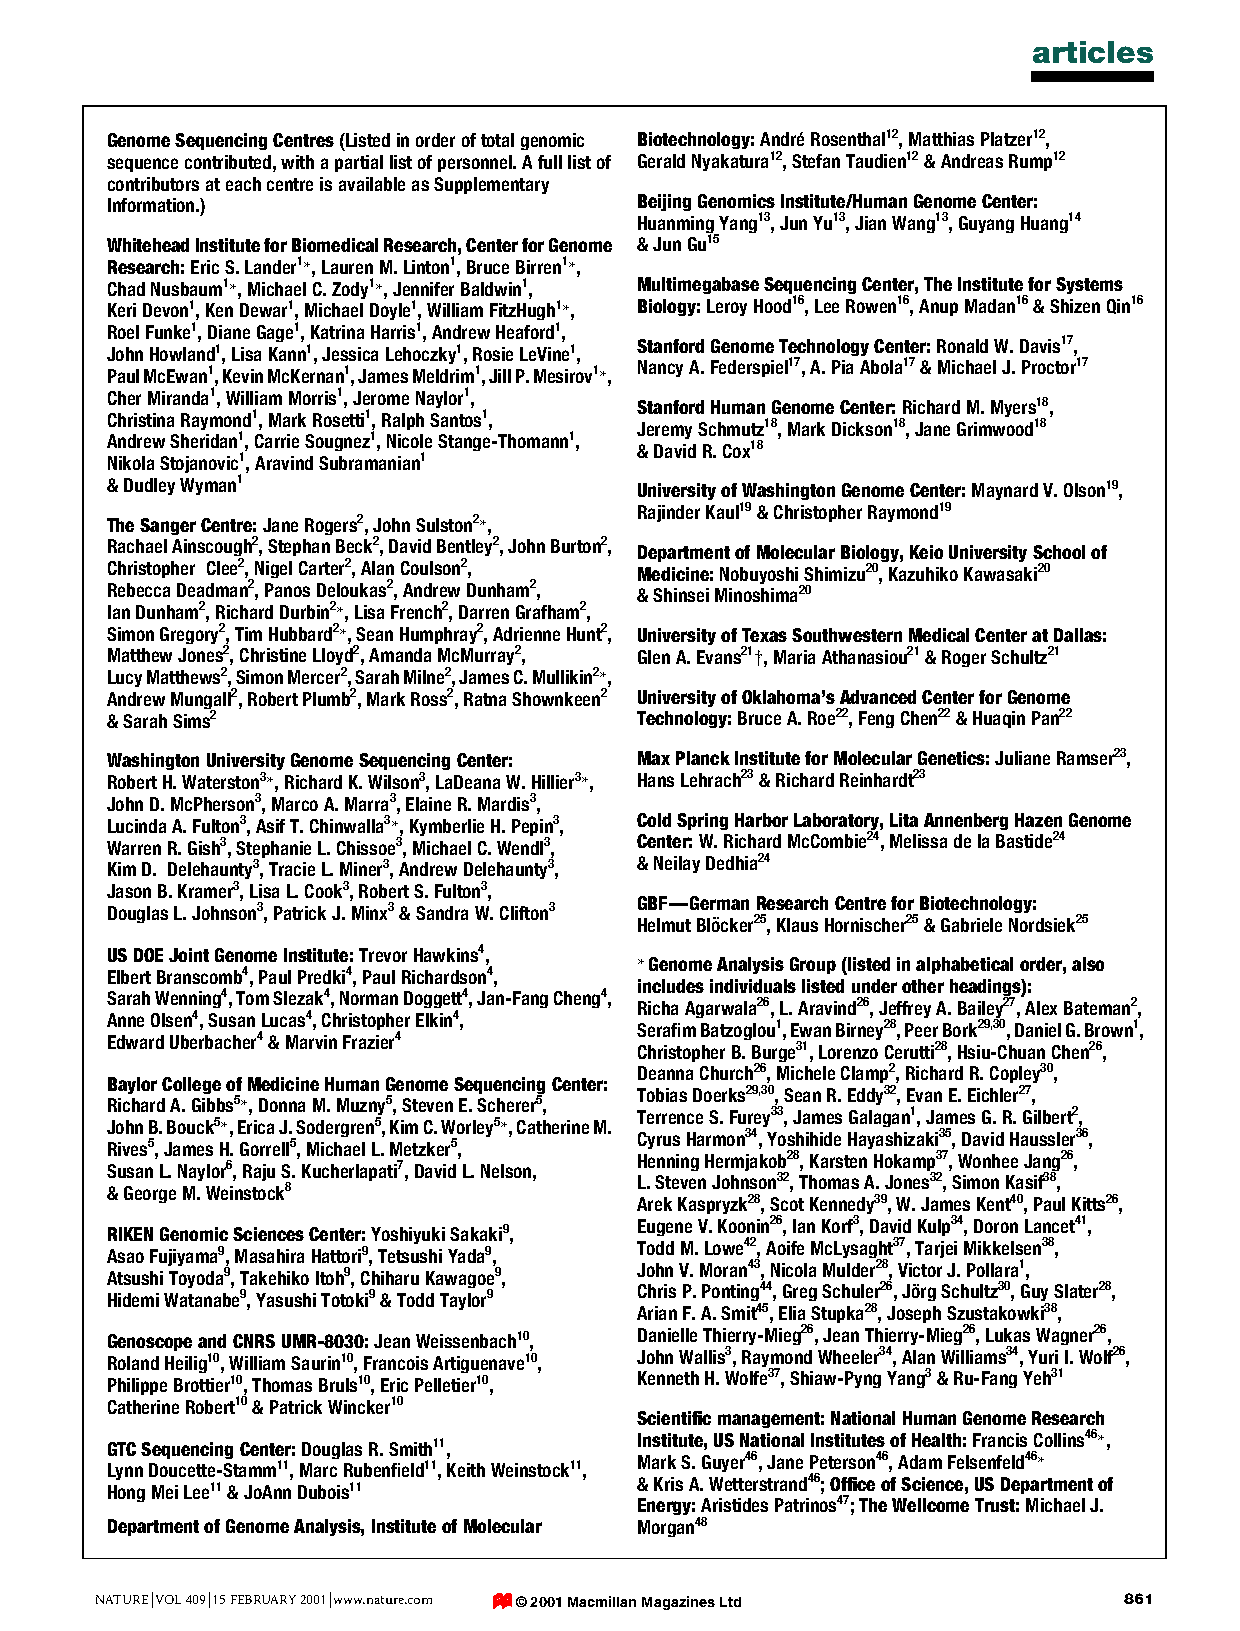
\includegraphics[height=\textheight]{figures/lander_initial_2001_authors}
\end{center}

\end{frame}
%%%%%%%%%%%%%%%%%%%%%%%%%%
\begin{frame}

\begin{center}
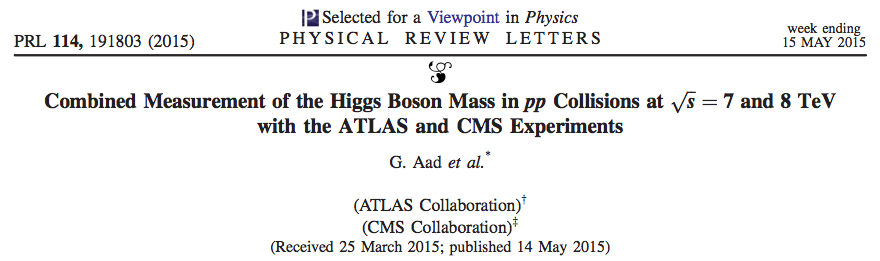
\includegraphics[width=\textwidth]{figures/aad_combined_2015_title}
\end{center}

\vfill
{\tiny \url{https://doi.org/10.1103/PhysRevLett.114.191803}}

\end{frame}
%%%%%%%%%%%%%%%%%%%%%%%%%%
\begin{frame}

\begin{center}
\includegraphics[height=\textheight]<1>{figures/aad_combined_2015_authors_01}
\includegraphics[height=\textheight]<2>{figures/aad_combined_2015_authors_02}
\includegraphics[height=\textheight]<3>{figures/aad_combined_2015_authors_03}
\includegraphics[height=\textheight]<4>{figures/aad_combined_2015_authors_04}
\includegraphics[height=\textheight]<5>{figures/aad_combined_2015_authors_05}
\includegraphics[height=\textheight]<6>{figures/aad_combined_2015_authors_06}
\includegraphics[height=\textheight]<7>{figures/aad_combined_2015_authors_07}
\includegraphics[height=\textheight]<8>{figures/aad_combined_2015_authors_08}
\includegraphics[height=\textheight]<9>{figures/aad_combined_2015_authors_09}
\includegraphics[height=\textheight]<10>{figures/aad_combined_2015_authors_10}
\includegraphics[height=\textheight]<11>{figures/aad_combined_2015_authors_11}
\includegraphics[height=\textheight]<12>{figures/aad_combined_2015_authors_12}
\includegraphics[height=\textheight]<13>{figures/aad_combined_2015_authors_13}
\includegraphics[height=\textheight]<14>{figures/aad_combined_2015_authors_14}
\includegraphics[height=\textheight]<15>{figures/aad_combined_2015_authors_15}
\includegraphics[height=\textheight]<16>{figures/aad_combined_2015_authors_16}
\includegraphics[height=\textheight]<17>{figures/aad_combined_2015_authors_17}
\includegraphics[height=\textheight]<18>{figures/aad_combined_2015_authors_18}
\includegraphics[height=\textheight]<19>{figures/aad_combined_2015_authors_19}
\includegraphics[height=\textheight]<20>{figures/aad_combined_2015_authors_20}
\includegraphics[height=\textheight]<21>{figures/aad_combined_2015_authors_21}
\includegraphics[height=\textheight]<22>{figures/aad_combined_2015_authors_22}
\includegraphics[height=\textheight]<23>{figures/aad_combined_2015_authors_23}
\includegraphics[height=\textheight]<24>{figures/aad_combined_2015_authors_24}
\includegraphics[height=\textheight]<25>{figures/aad_combined_2015_authors_25}
\end{center}

\end{frame}
%%%%%%%%%%%%%%%%%%%%%%%%%
\begin{frame}

\begin{center}
\Large{Fragile Families Challenge} \pause
\end{center}
A scientific mass collaboration combining \pause
\begin{itemize}
\item predictive modeling,\pause 
\item causal inference, \pause 
\item and in-depth qualitative interviews 
\end{itemize}
\pause to improve the lives of disadvantaged children in the US.  

\end{frame}
%%%%%%%%%%%%%%%%%%%%%%%%%%%
\begin{frame}

\begin{center}

\includegraphics[width=\textwidth]{figures/ff_logo}
\end{center}

\begin{itemize}
\item Birth cohort panel study
\item $\approx$ 5,000 children born in 20 U.S. cities
\item Followed from birth through age 15
\end{itemize}

\textcolor{blue}{Key research question}: What can be done to improve the life chances of disadvantaged children?

\end{frame}
%%%%%%%%%%%%%%%%%%%%%%%%%%%
\begin{frame}

Hundreds of papers and dozens of dissertations \vskip 1cm
\scriptsize \url{http://crcw.princeton.edu/publications/publications.asp}

\end{frame}
%%%%%%%%%%%%%%%%%%%%%%%%%%
\begin{frame}

\begin{center}
\large{Social Scientists $\longleftrightarrow$ Data Scientists}
\end{center}
\pause
\begin{center}
\LARGE{
$\hat{\beta} \quad \& \quad \hat{y}$
}
\end{center}

\vfill
Mullainathan and Spiess (2017): \url{http://dx.doi.org/10.1257/jep.31.2.87}
\end{frame}
%%%%%%%%%%%%%%%%%%%%%%%%%
\begin{frame}

\begin{center}
\only<1>{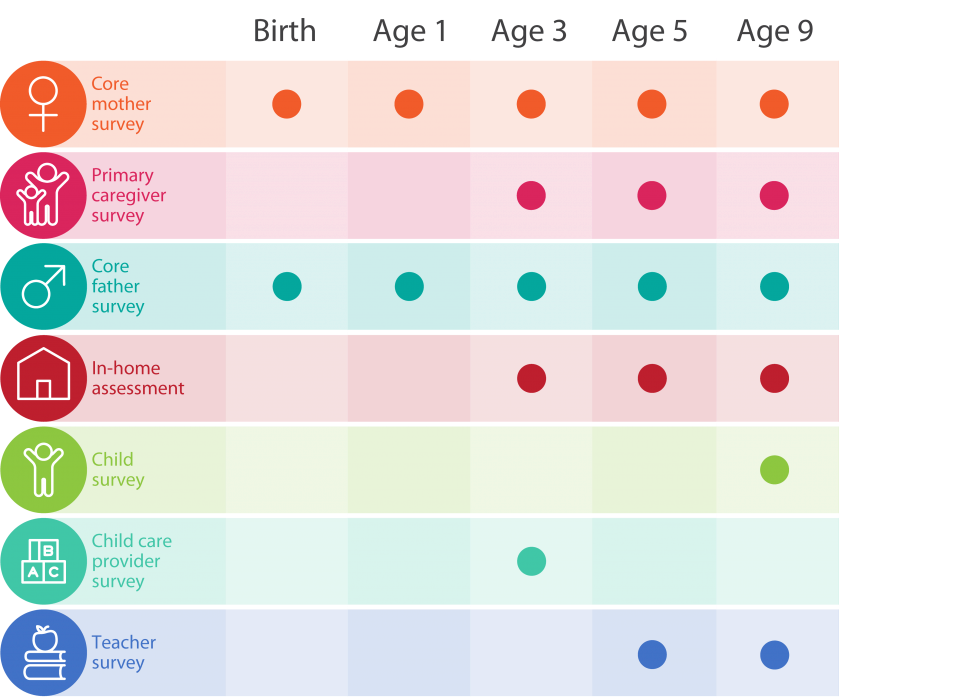
\includegraphics[width=\textwidth]{figures/ff_design_public_b9}}
\only<2>{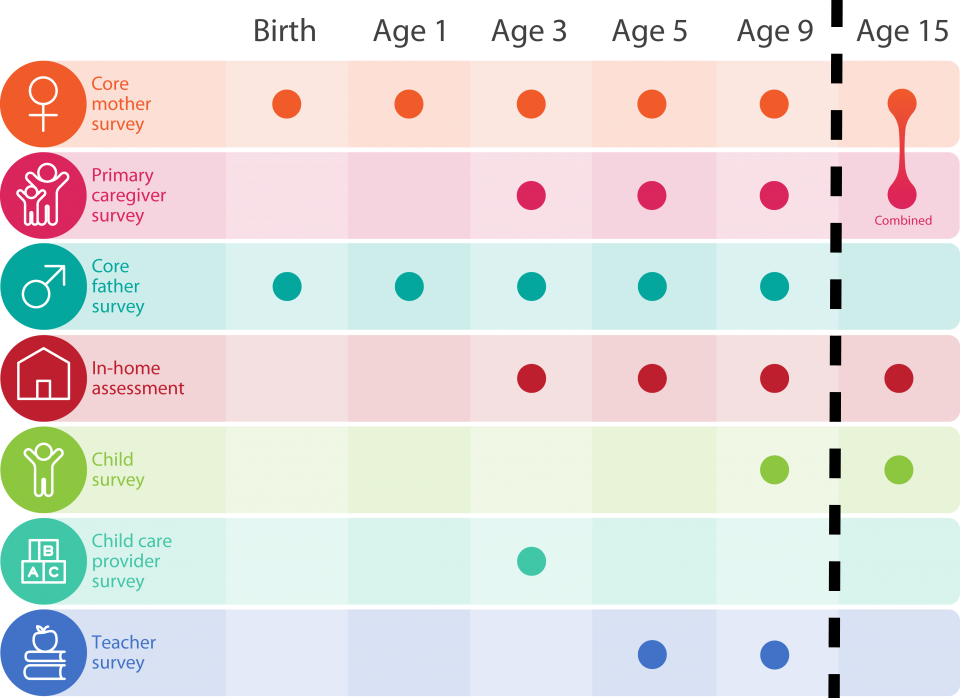
\includegraphics[width=\textwidth]{figures/ff_design_public2}}
\end{center}

\end{frame}
%%%%%%%%%%%%%%%%%%%%%%%%%
\begin{frame}

\begin{center}
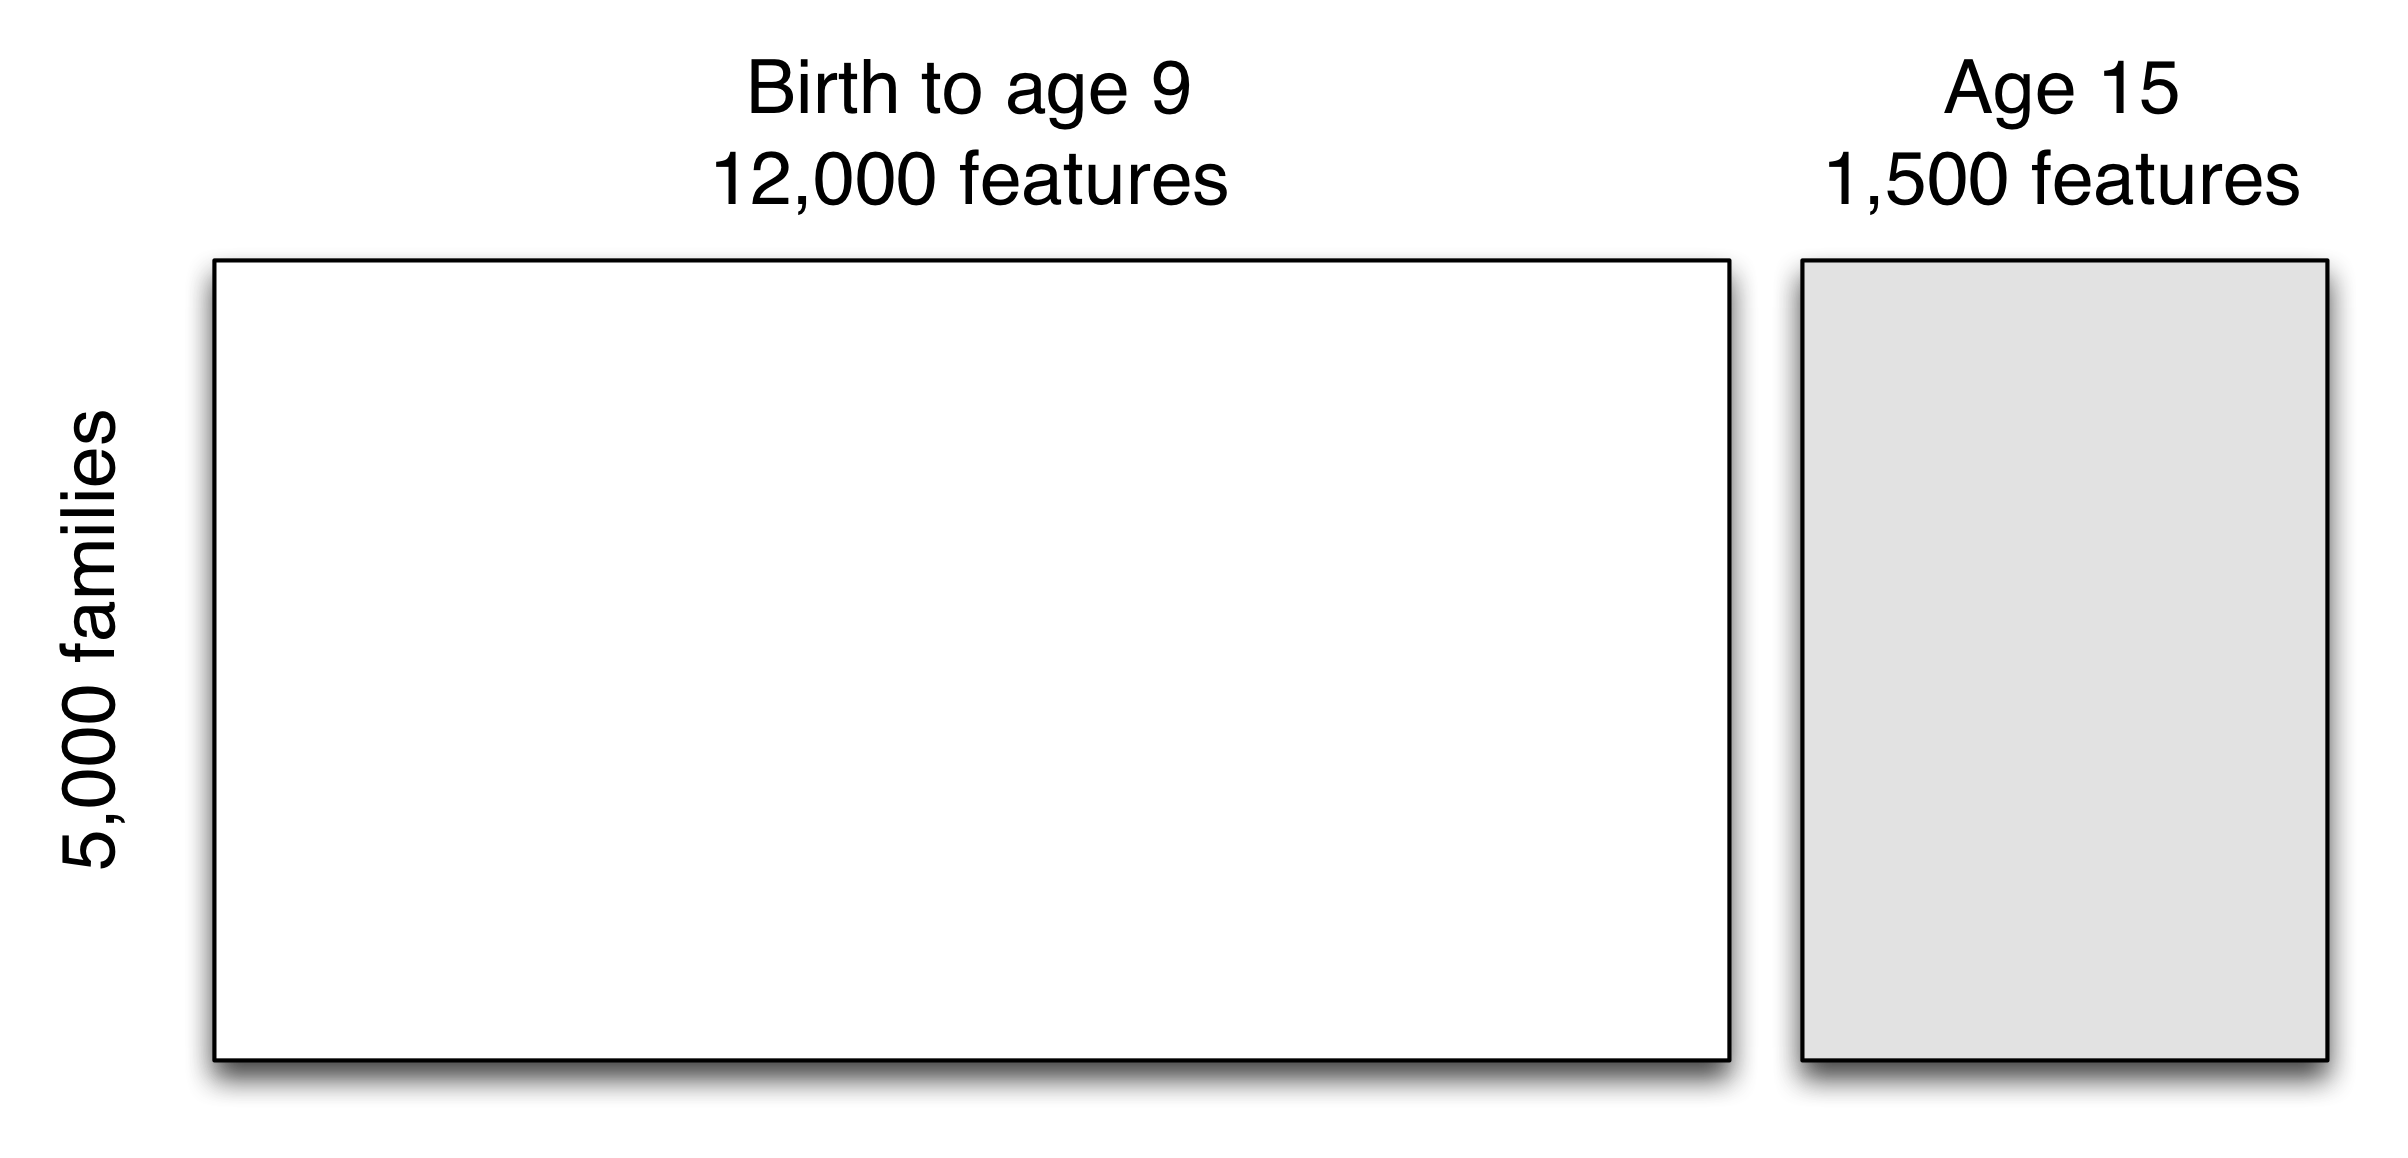
\includegraphics[width=\textwidth]{figures/ff_design_matrix_ml}
\end{center}

\end{frame}
%%%%%%%%%%%%%%%%%%%%%%%%%
\begin{frame}

\begin{center}
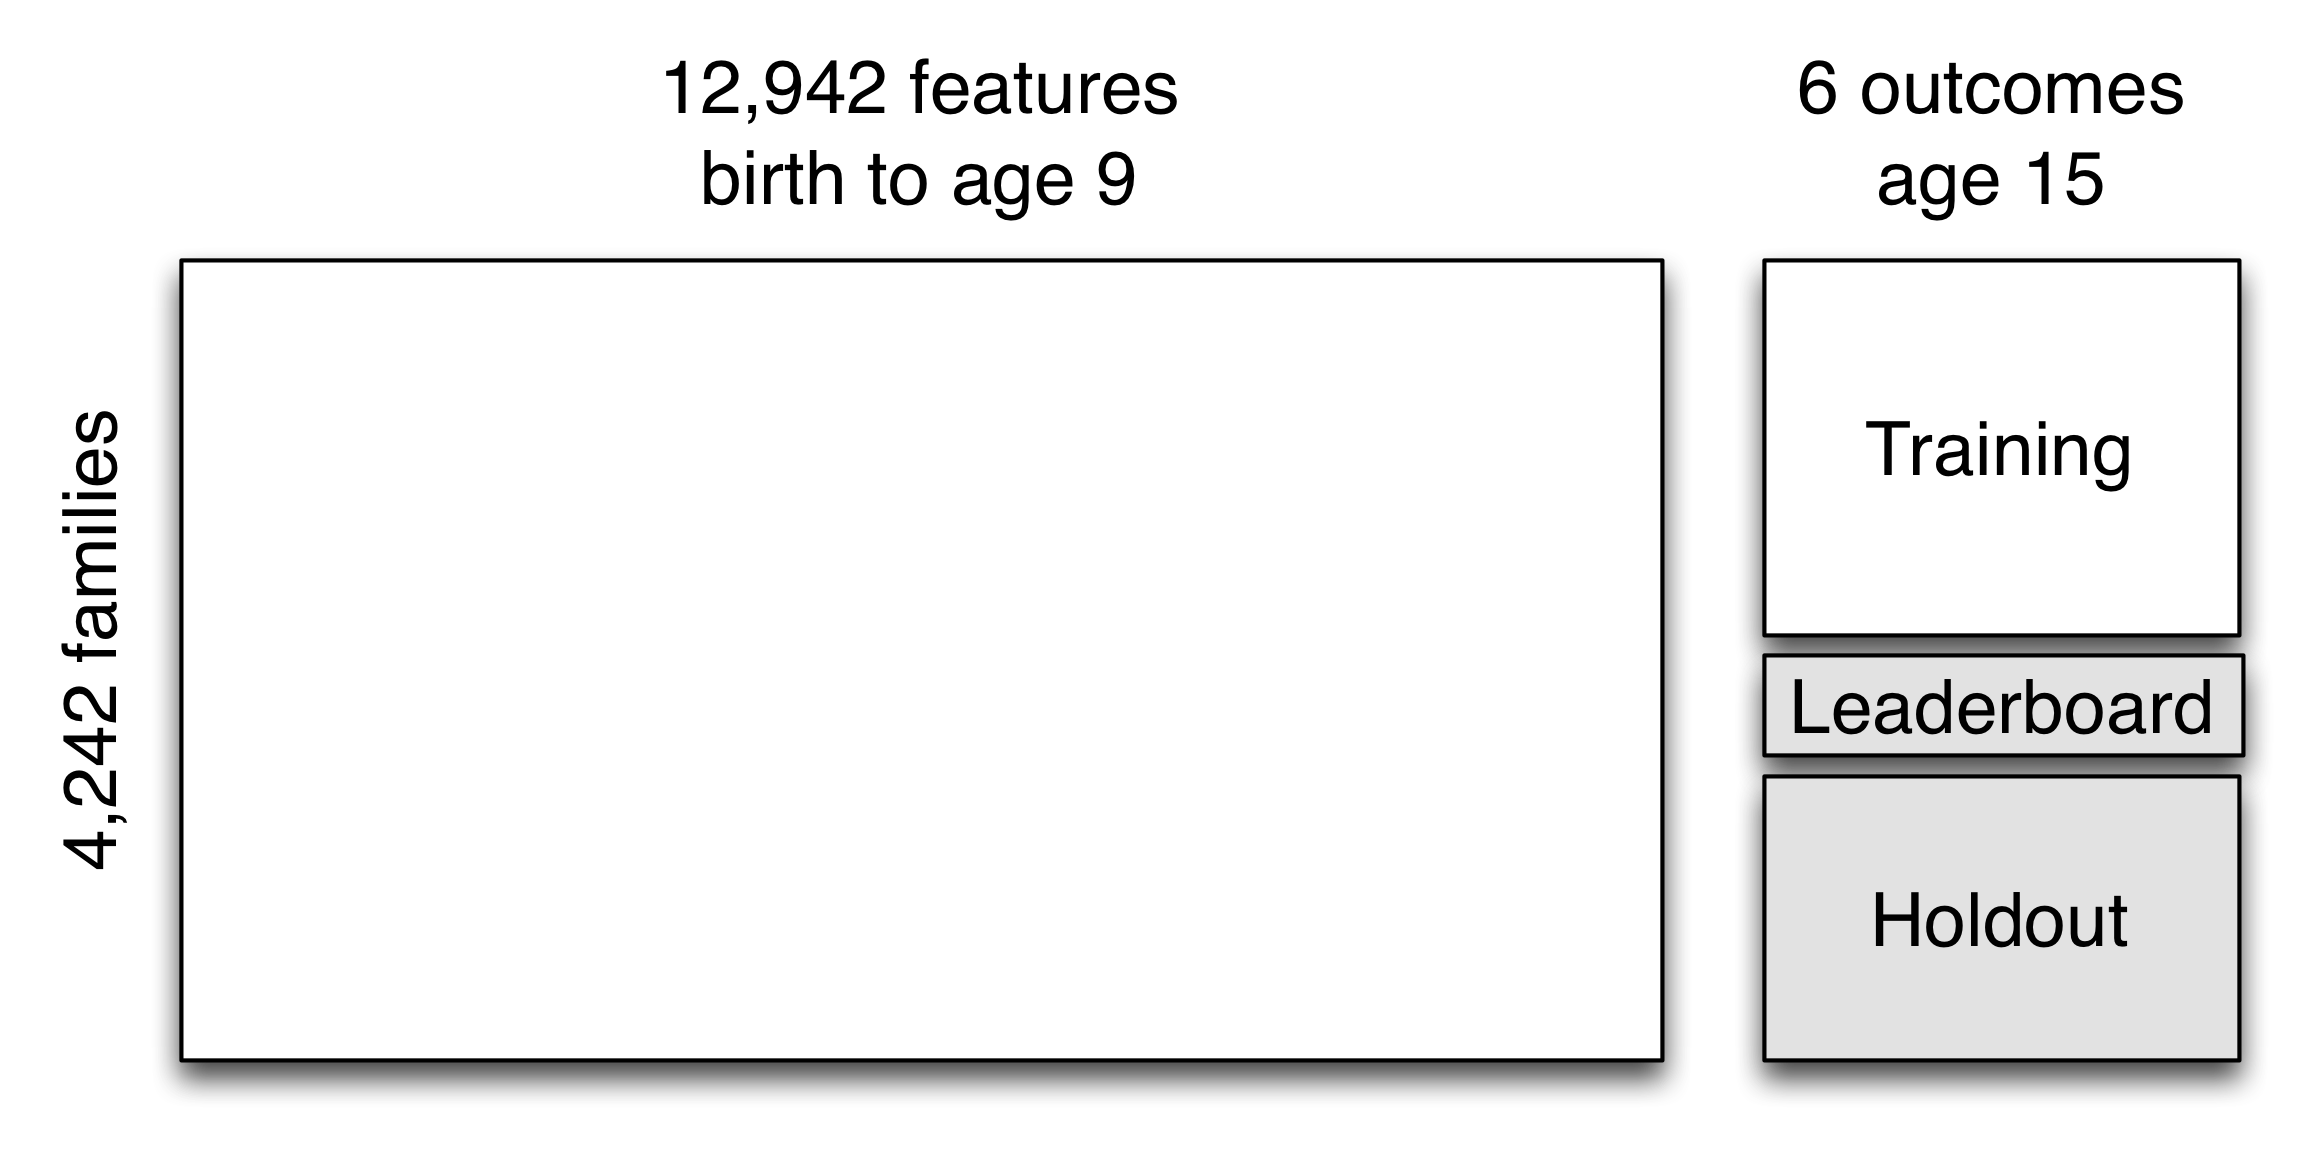
\includegraphics[width=\textwidth]{figures/ffc_design_matrix_ml}
\end{center}

\end{frame}
%%%%%%%%%%%%%%%%%%%%%%%%%
\begin{frame}

\begin{tabular}{p{.4\textwidth}p{.4\textwidth}}
Continuous outcomes:
\begin{itemize}
\item GPA
\item Grit
\item Material hardship
\end{itemize}
&
Binary outcomes:
\begin{itemize}
\item Housing eviction
\item Layoff of a caregiver
\item Job training for a caregiver
\end{itemize}
\end{tabular}

\end{frame}
%%%%%%%%%%%%%%%%%%%%%%%%%
\begin{frame}

Fragile Families Challenge:
\begin{enumerate}
\item common task method
\pause
\item use submissions to do cool stuff
\end{enumerate}

\end{frame}
%%%%%%%%%%%%%%%%%%%%%%%%%
\begin{frame}

What has happened so far?\\ \pause
\begin{itemize}
\item Launched one year ago \pause
\item Hundreds of participants from around the world (undergrads, grad students, and professionals) \pause
\item Results were . . . . disappointing to me (talk summarizing the results: \textcolor{blue}{\url{https://youtu.be/HrYPtdXeSaM}}). \pause
\item Why were the results disappointing?
\end{itemize}

\end{frame}
%%%%%%%%%%%%%%%%%%%%%%%%%
\begin{frame}

Why should we care about the predictability of social outcomes?
\begin{itemize}
\item Scientific reasons \pause
\item Policy reasons
\end{itemize}

\begin{center}
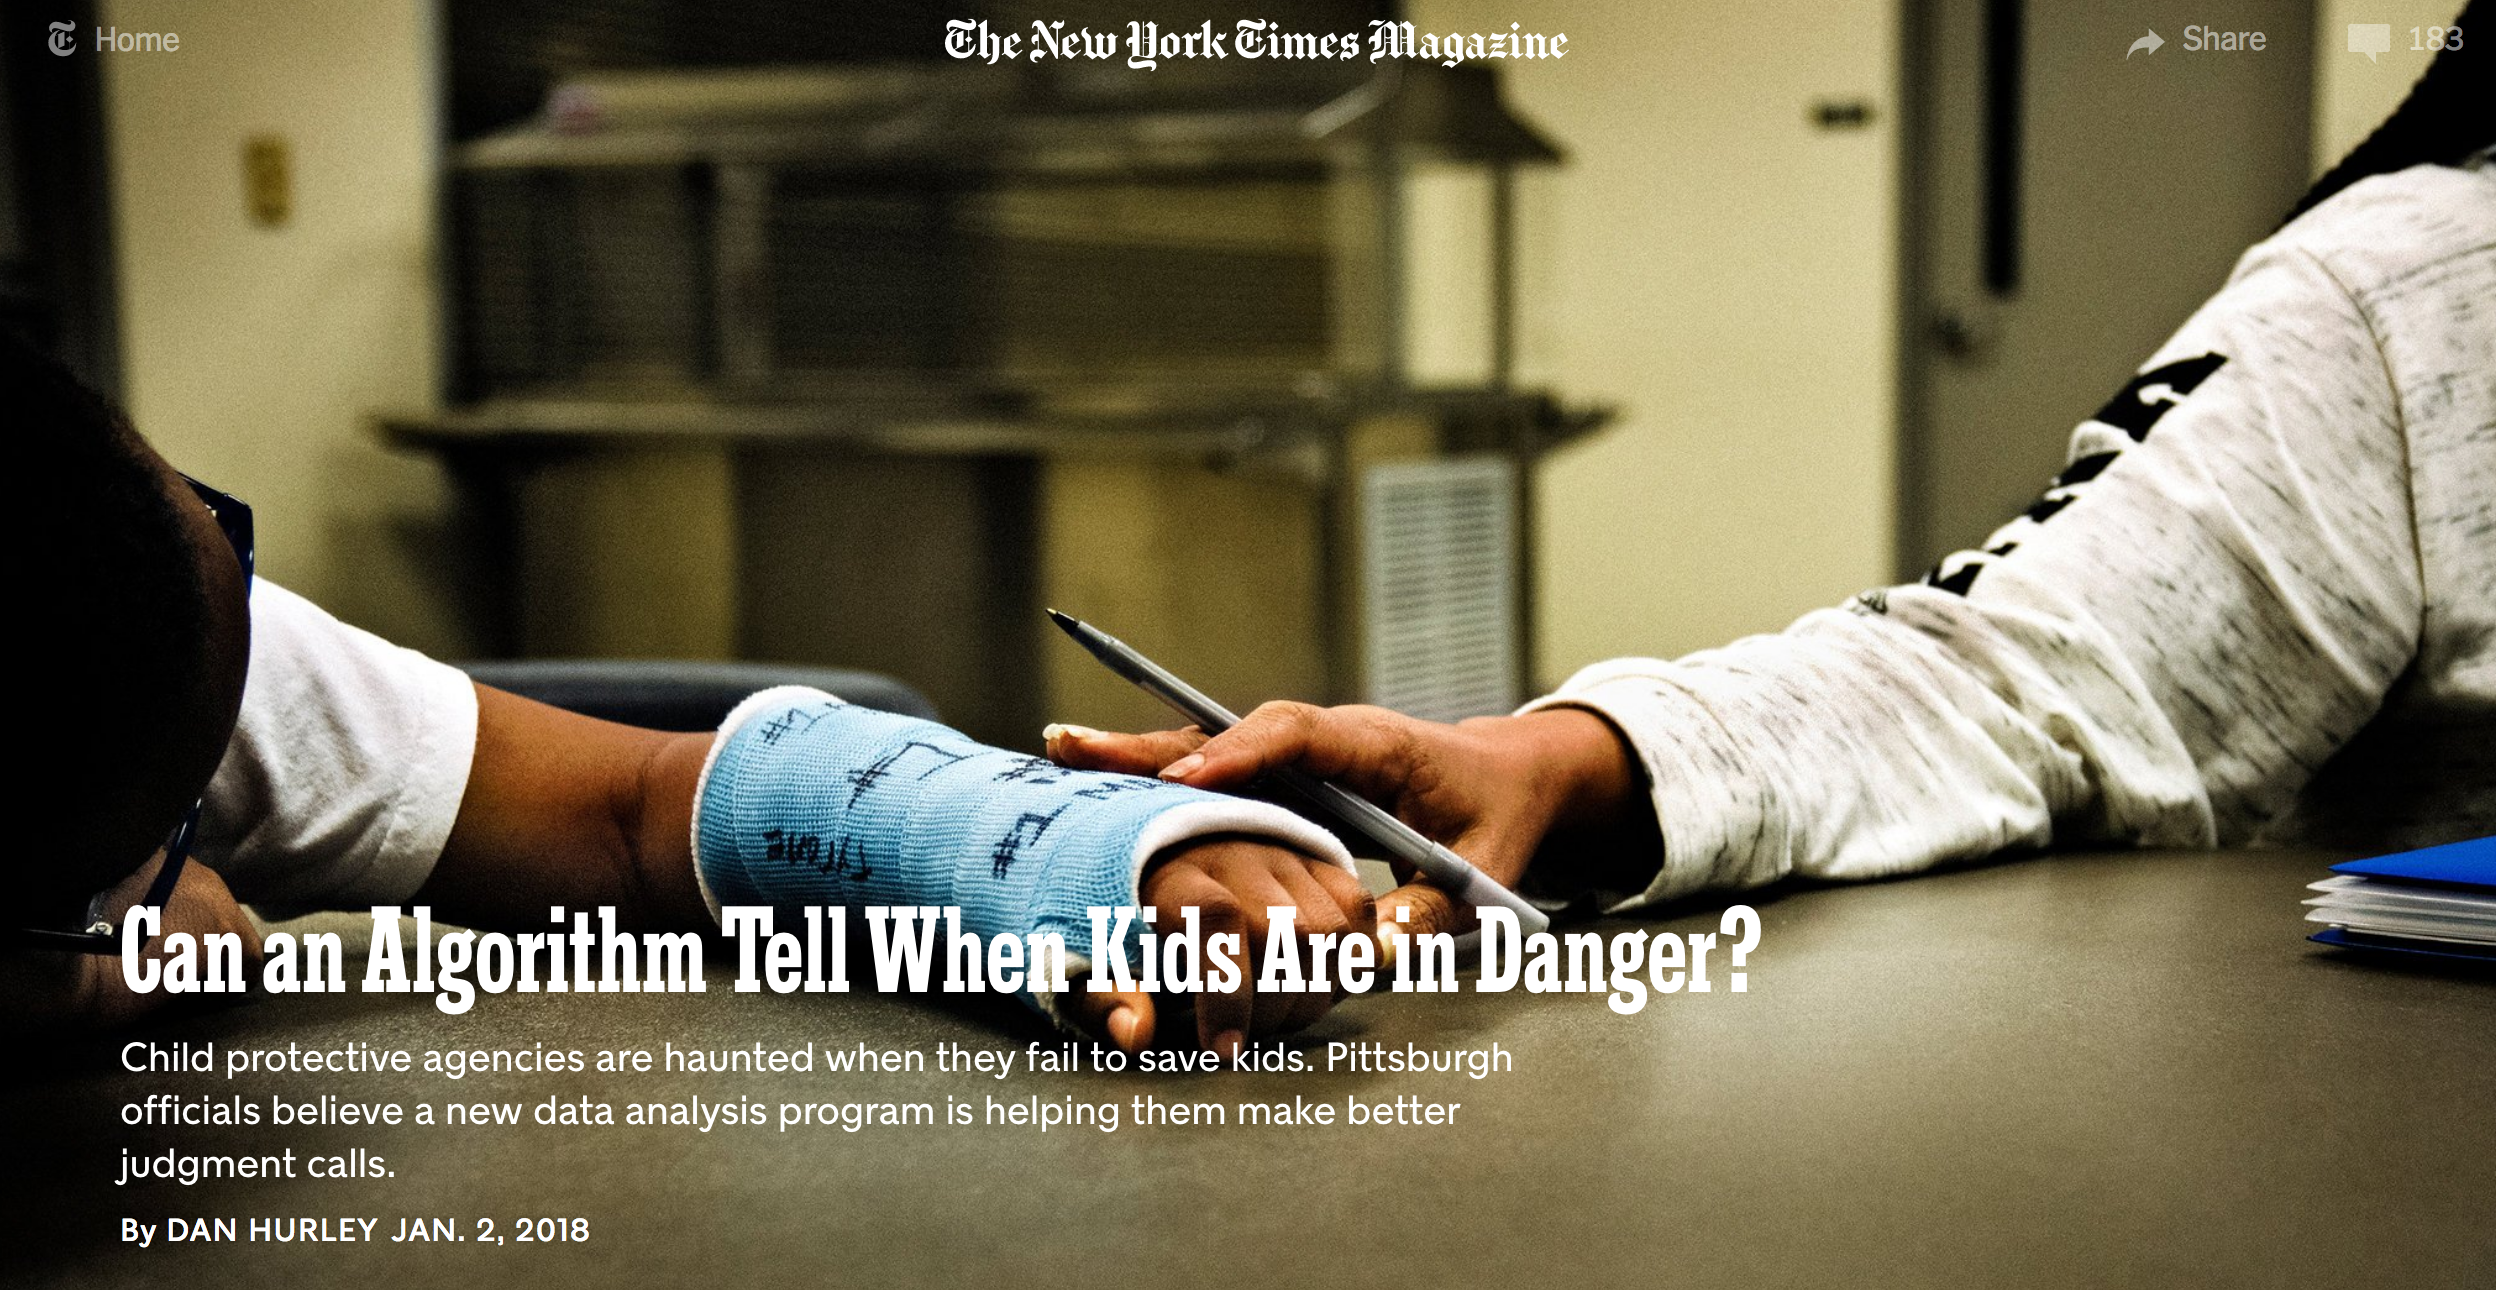
\includegraphics[width=0.8\textwidth]{figures/hurley_can_2018_title}
\end{center}

\vfill

We need to understand the strengths \emph{and} weakness of predictive models of social behavior
\end{frame}
%%%%%%%%%%%%%%%%%%%%%%%%%
\begin{frame}

\begin{itemize}
\item A team of people\footnote{Alexander Kindel, Vineet Bansal, Kristin Catena, Thomas Hartshorne, Kate Jaeger, Dawn Koffman, Sara McLanahan, Maya Phillips, Shiva Rouhani, Ryan Vinh, Matthew Salganik.} has spent months making the data easier to use. \pause
\item Is it possible to do better than last time? Or, is there a fundamental limit with this data and this task? \pause
\item Let's see if it improves performance, \pause and let's see if you can help make this easier for future researchers.
\end{itemize}

\end{frame}
%%%%%%%%%%%%%%%%%%%%%%%%%
\section{How to participate}
%%%%%%%%%%%%%%%%%%%%%%%%%
\begin{frame}

\large{
\begin{center}
How to participate\\
\textcolor{blue}{\href{https://codalab.fragilefamilieschallenge.org/competitions/23}{https://codalab.fragilefamilieschallenge.org/competitions/23}}
\end{center}
}

\end{frame}
%%%%%%%%%%%%%%%%%%%%%%%%%
\begin{frame}

\Large{
\begin{center}
Introducing the outcome variables
\end{center}
}

\end{frame}
%%%%%%%%%%%%%%%%%%%%%%%%%
\begin{frame}

\Large{
\begin{center}
GPA\footnote{Learn more at \url{http://www.fragilefamilieschallenge.org/gpa/} \vskip .2cm}
\pause \vskip .5cm
How do kids beat the odds academically?
\end{center}
}

\end{frame}
%%%%%%%%%%%%%%%%%%%%%%%%%
\begin{frame}{GPA\footnote{This variable is reverse-coded in the data file so that higher values represent higher GPAs.}}

\centering
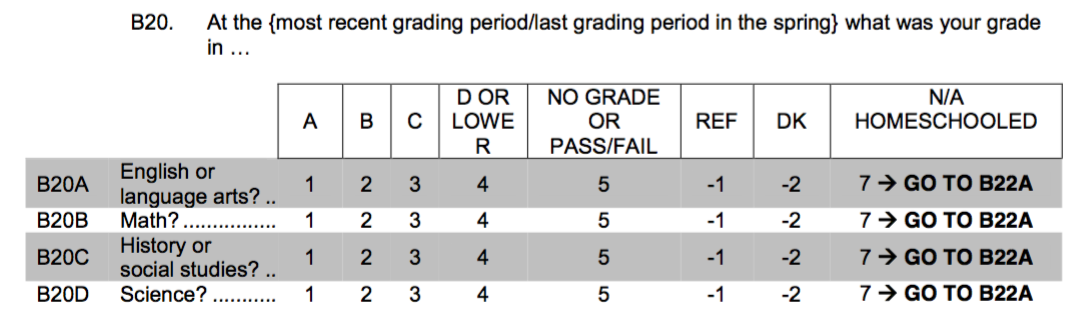
\includegraphics[width = .9\textwidth]{figures/GPA_questionnaire}

\end{frame}
%%%%%%%%%%%%%%%%%%%%%%%%%
\begin{frame}

\centering
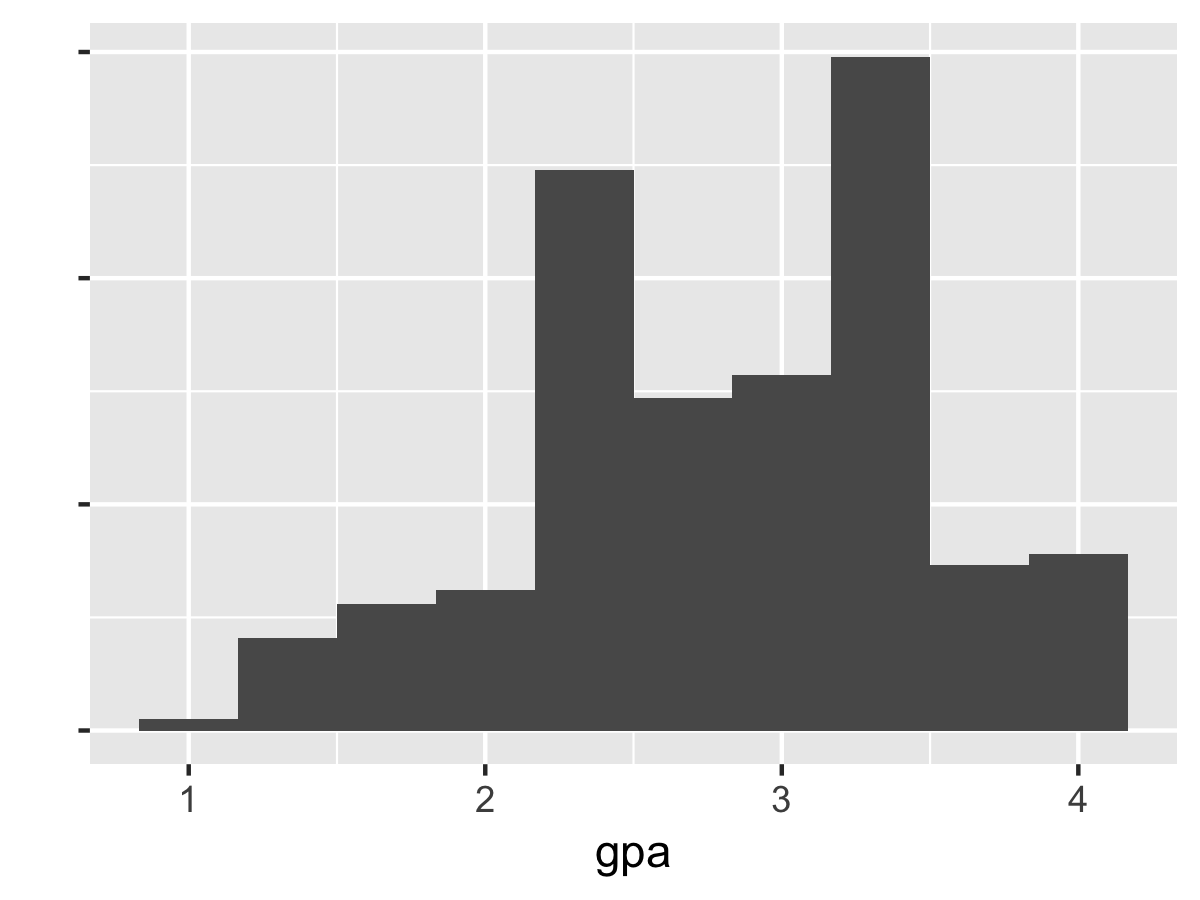
\includegraphics[width = .9\textwidth]{figures/gpaDist}

\end{frame}
%%%%%%%%%%%%%%%%%%%%%%%%%
\begin{frame}
\begin{center}
\Large{
``Grit'' predicts success, possibly more than IQ.\footnote{Learn more at \url{http://www.fragilefamilieschallenge.org/grit/}\vskip .2cm} \vskip .3cm

\includegraphics[width = .3\textwidth]{figures/duckworth_grit_2016_cover} \vskip .3cm \pause
What makes some kids gritty?
} 
\end{center}
\end{frame}
%%%%%%%%%%%%%%%%%%%%%%%%%%%
\begin{frame}{Grit\footnote{This variable is reverse-coded in the data file so that higher values represent more grit.}}

\centering
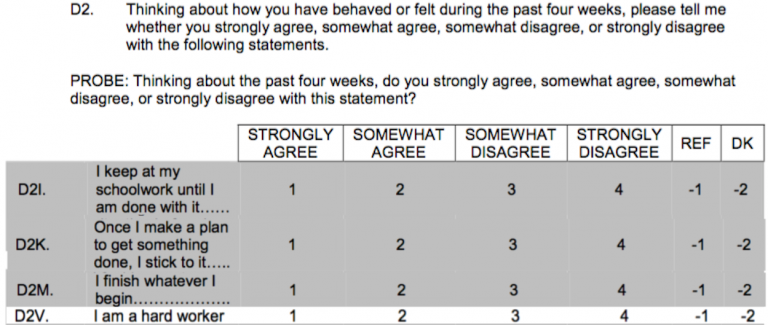
\includegraphics[width = .9\textwidth]{figures/grit_questionnaire2}

\end{frame}
%%%%%%%%%%%%%%%%%%%%%%%%%
\begin{frame}

\centering
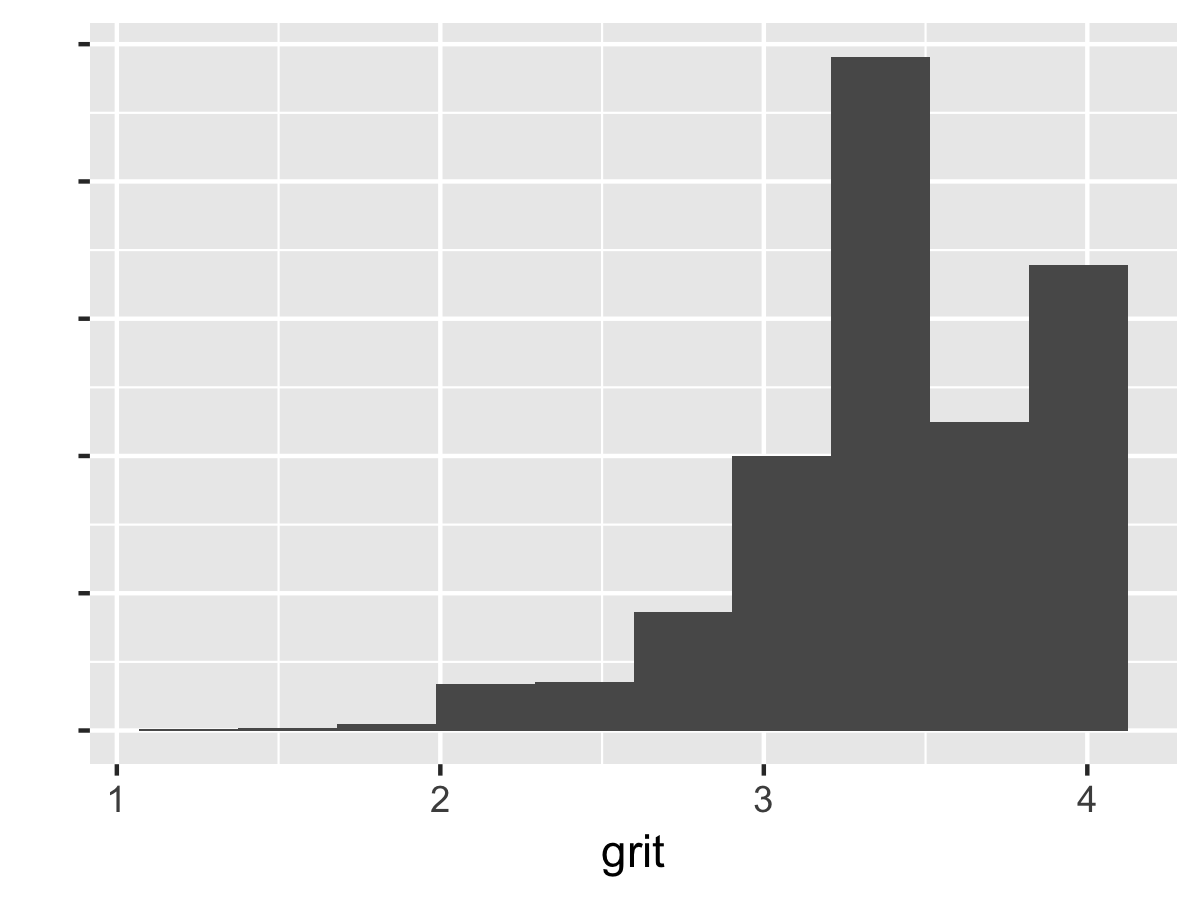
\includegraphics[width = .9\textwidth]{figures/gritDist}

\end{frame}
%%%%%%%%%%%%%%%%%%%%%%%%%
\begin{frame}

\Large{
\begin{center}
Material hardship\footnote{Learn more at \url{http://www.fragilefamilieschallenge.org/material-hardship/}\vskip .2cm} \pause \vskip .3cm 
What unmeasured predictors are associated with families unexpectedly escaping severe deprivation? 
\pause \vskip .3cm What sends families unexpectedly into deep poverty?
\end{center}
}

\end{frame}
%%%%%%%%%%%%%%%%%%%%%%%%%%%
\begin{frame}{Material hardship}

\centering
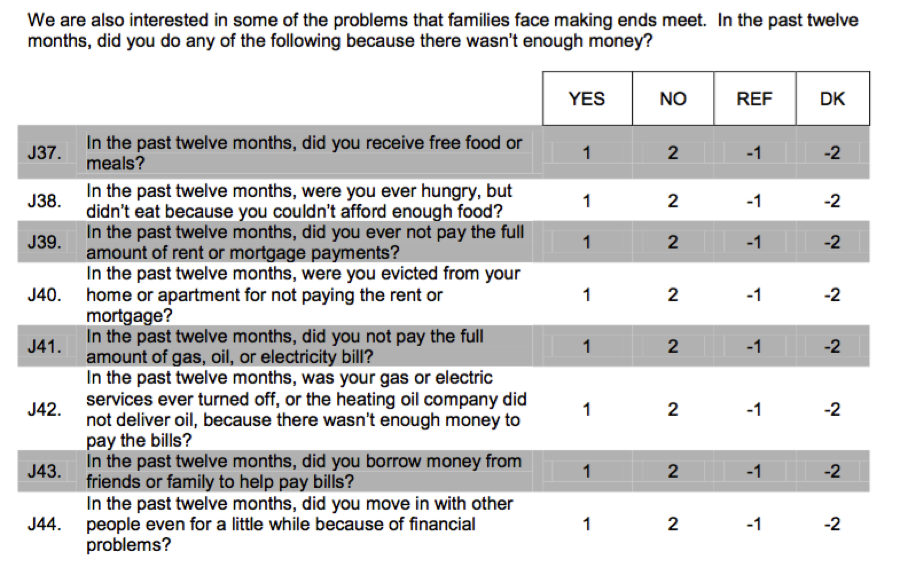
\includegraphics[width = .9\textwidth]{figures/materialHardship_questionnaireA}

\end{frame}
%%%%%%%%%%%%%%%%%%%%%%%%%%%
\begin{frame}{Material hardship}

\centering
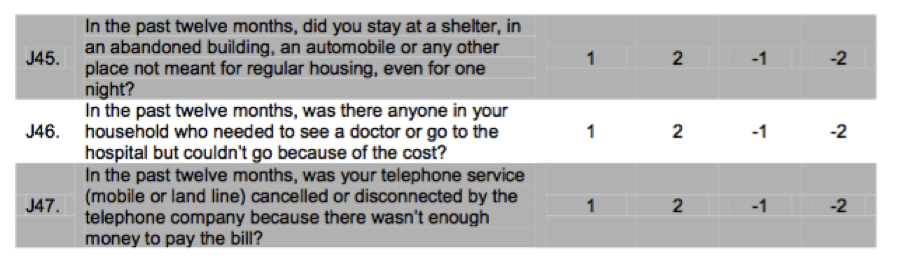
\includegraphics[width = .9\textwidth]{figures/materialHardship_questionnaireB}

\end{frame}
%%%%%%%%%%%%%%%%%%%%%%%%%
\begin{frame}

\centering
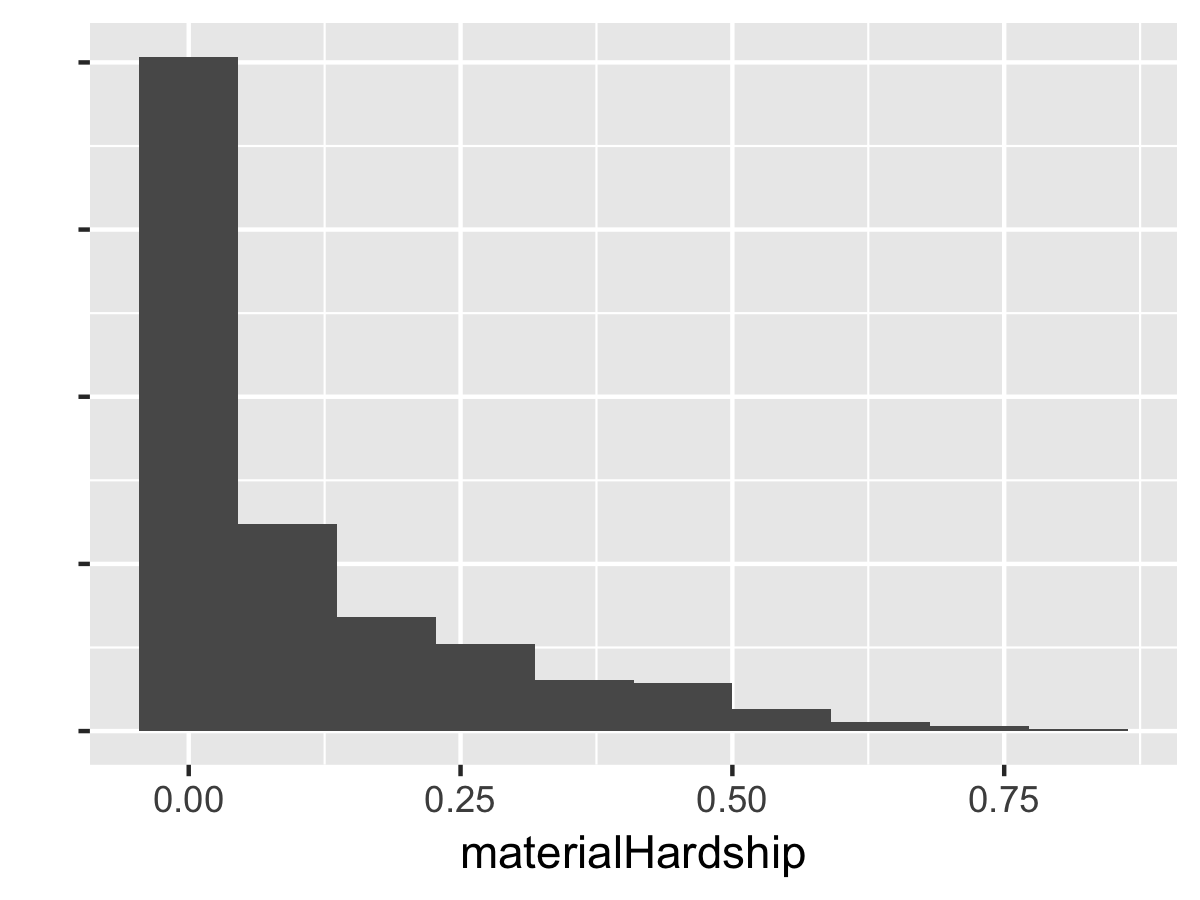
\includegraphics[width = .9\textwidth]{figures/materialHardshipDist}

\end{frame}
%%%%%%%%%%%%%%%%%%%%%%%%%
\begin{frame}

\Large{
\begin{center}
Eviction\footnote{Learn more at \url{http://www.fragilefamilieschallenge.org/eviction/}\vskip .2cm}
\pause \vskip .5cm
Does housing eviction \textbf{cause} worse outcomes as kids transition to adulthood?\footnote{Note: You will just create propensity scores for eviction given background variables; causal inference comes in the second stage of the Challenge when outcomes are measured several years from now.}
\end{center}
}

\end{frame}
%%%%%%%%%%%%%%%%%%%%%%%%%%%
\begin{frame}{Eviction}

\centering
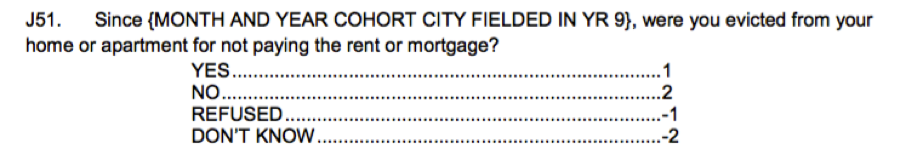
\includegraphics[width = .9\textwidth]{figures/eviction_questionnaire}

\end{frame}
%%%%%%%%%%%%%%%%%%%%%%%%%
\begin{frame}

\centering
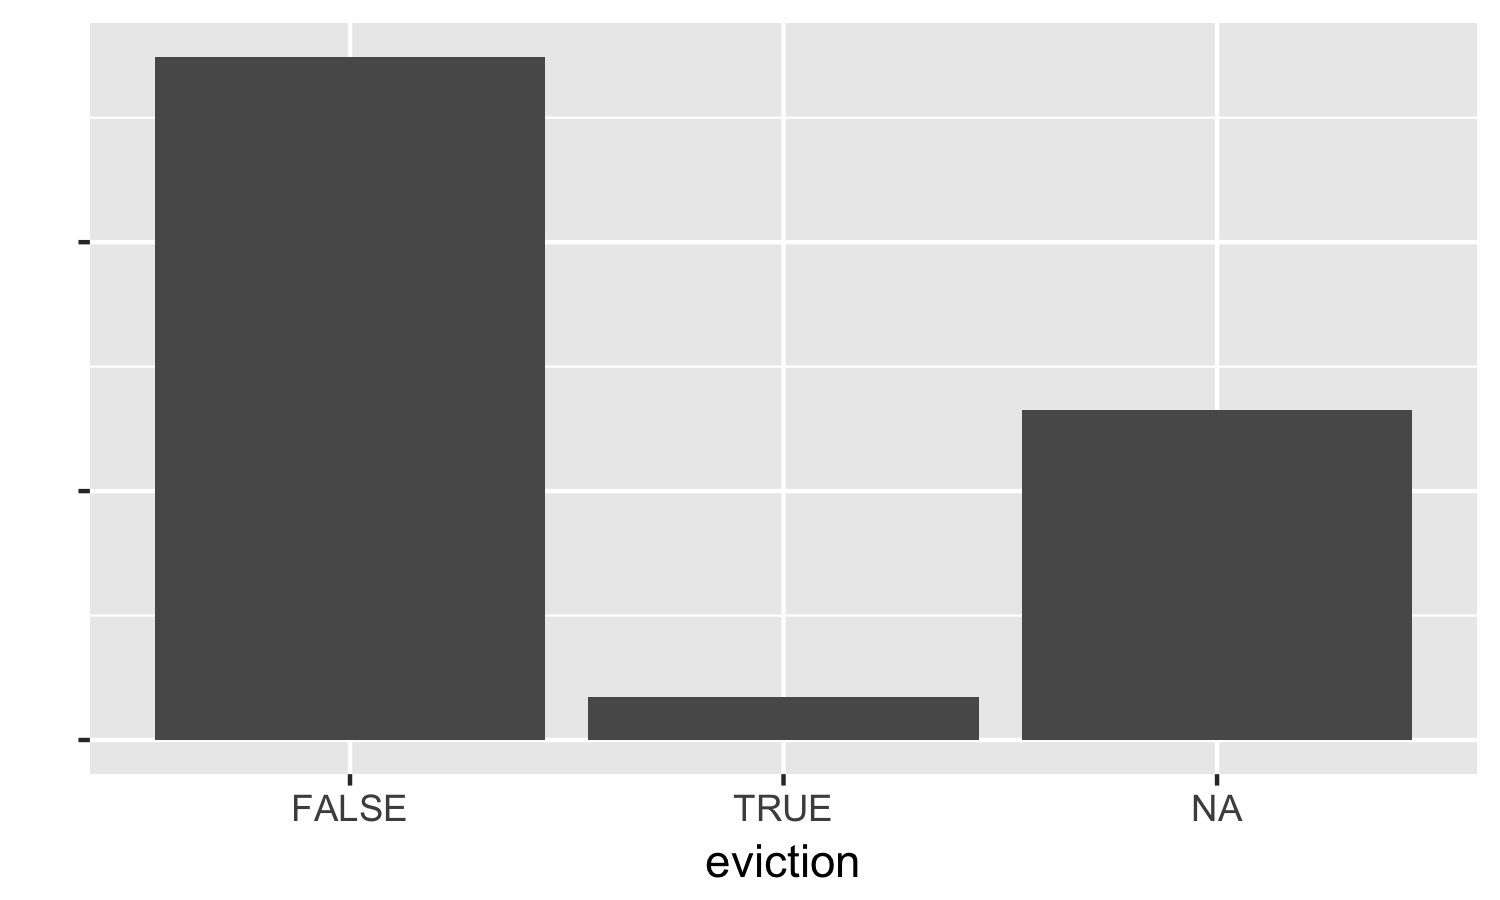
\includegraphics[width = .9\textwidth]{figures/evictionDist}

\end{frame}
%%%%%%%%%%%%%%%%%%%%%%%%%
\begin{frame}

\Large{
\begin{center}
Caregiver layoff\footnote{Learn more at \url{http://www.fragilefamilieschallenge.org/layoff/}\vskip .2cm}
\pause \vskip .5cm 
Does layoff of a caregiver \textbf{cause} collateral damage for kids?\footnote{Note: You will just create propensity scores for caregiver layoff given background variables; causal inference comes in the second stage of the Challenge when outcomes are measured several years from now.}
\end{center}
}

\end{frame}
%%%%%%%%%%%%%%%%%%%%%%%%%%%
\begin{frame}{Caregiver layoff}

\centering
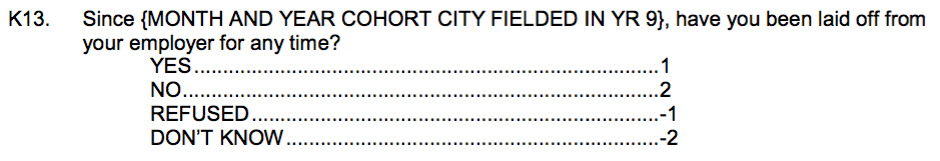
\includegraphics[width = .9\textwidth]{figures/layoff_questionnaire}

\end{frame}
%%%%%%%%%%%%%%%%%%%%%%%%%
\begin{frame}

\centering
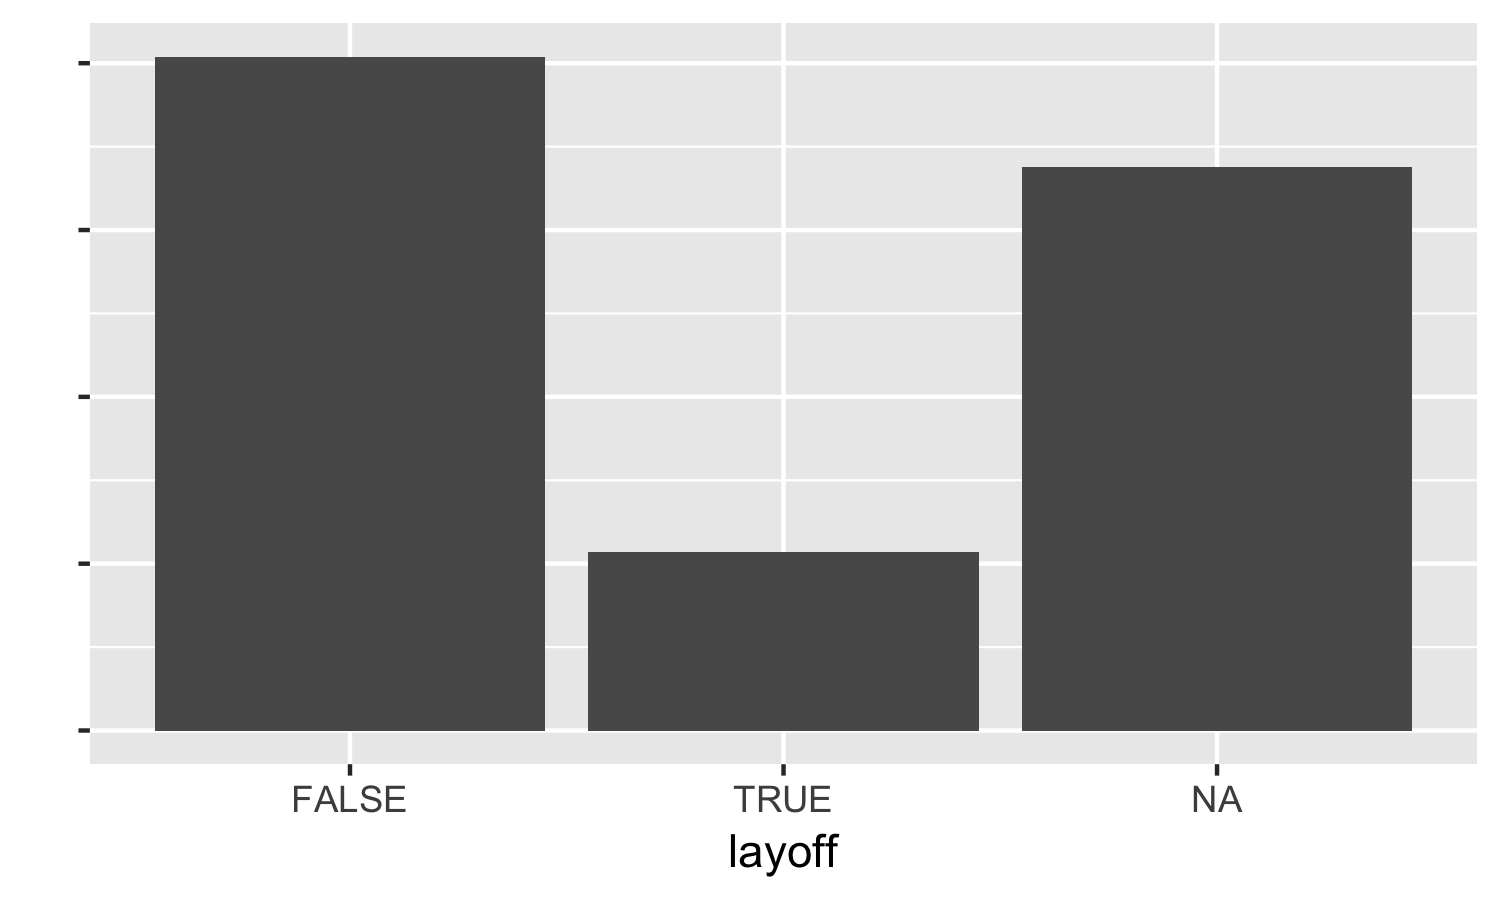
\includegraphics[width = .9\textwidth]{figures/layoffDist}

\end{frame}
%%%%%%%%%%%%%%%%%%%%%%%%%
\begin{frame}

\Large{
\begin{center}
Job training\footnote{Learn more at \url{http://www.fragilefamilieschallenge.org/job-training/}\vskip .2cm}
\pause \vskip .5cm 
Does job training for a caregiver \textbf{cause} collateral benefits for children?\footnote{Note: You will just create propensity scores for job training given background variables; causal inference comes in the second stage of the Challenge when outcomes are measured several years from now.}
\end{center}
}

\end{frame}
%%%%%%%%%%%%%%%%%%%%%%%%%%%
\begin{frame}{Caregiver job training}

\centering
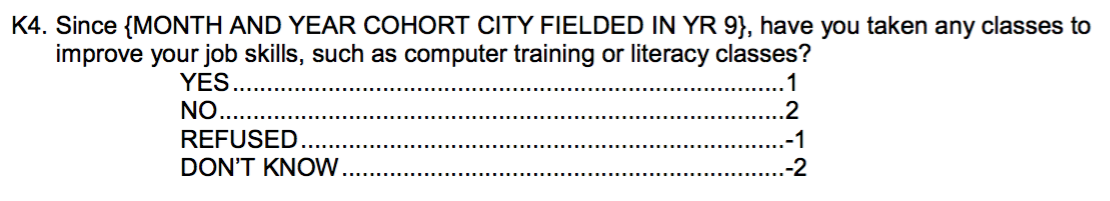
\includegraphics[width = .9\textwidth]{figures/jobTraining_questionnaire}

\end{frame}
%%%%%%%%%%%%%%%%%%%%%%%%%
\begin{frame}

\centering
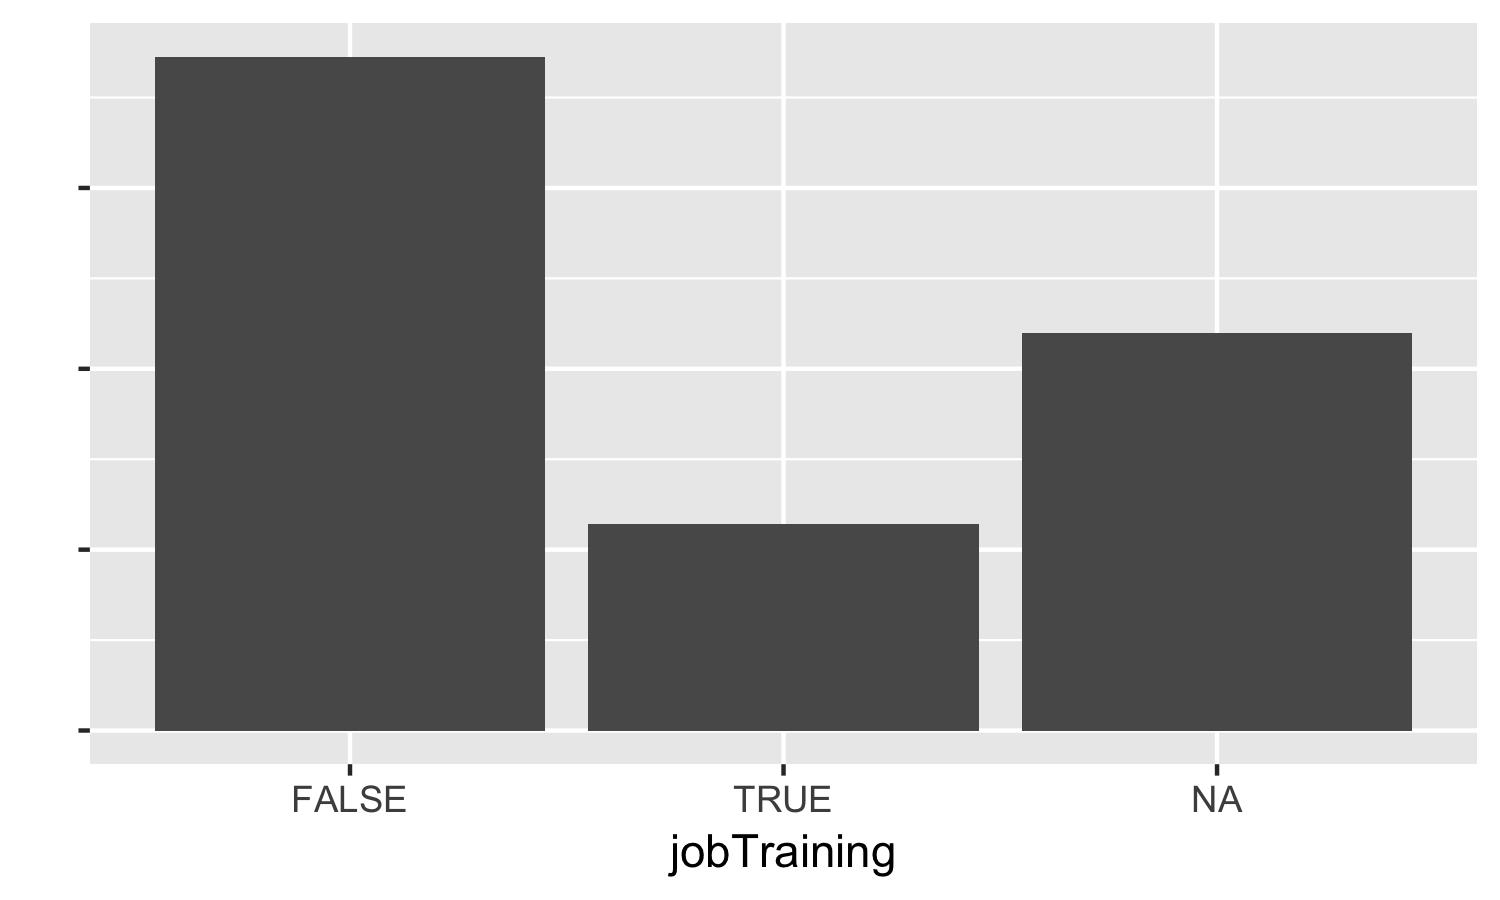
\includegraphics[width = .9\textwidth]{figures/jobTrainingDist}

\end{frame}
%%%%%%%%%%%%%%%%%%%%%%%%%%%
\begin{frame}

\Large{
\begin{center}
Introducing the data
\end{center}
}

\end{frame}
%%%%%%%%%%%%%%%%%%%%%%%%%
\begin{frame}

\textbf{The Fragile Families and Child Wellbeing Study is a dataset of real people who have selflessly opened up their lives to us for the last 15 years so that their experiences can contribute to scientific research. By participating in the Fragile Families Challenge, you become a collaborator in this project. It is of the utmost importance that you respect the families in the data by using what they have told us responsibly.}

\end{frame}
%%%%%%%%%%%%%%%%%%%%%%%%%
\begin{frame}

\begin{itemize}
\item Before you have access to the data, you will sign a data use agreement
\pause
\item After this activity you will delete the data from your computer
\pause
\item If you want to keep working with the data afterwards, you can apply for access through the Fragile Families website
\end{itemize}

\end{frame}
%%%%%%%%%%%%%%%%%%%%%%%%
\begin{frame}

\begin{center}
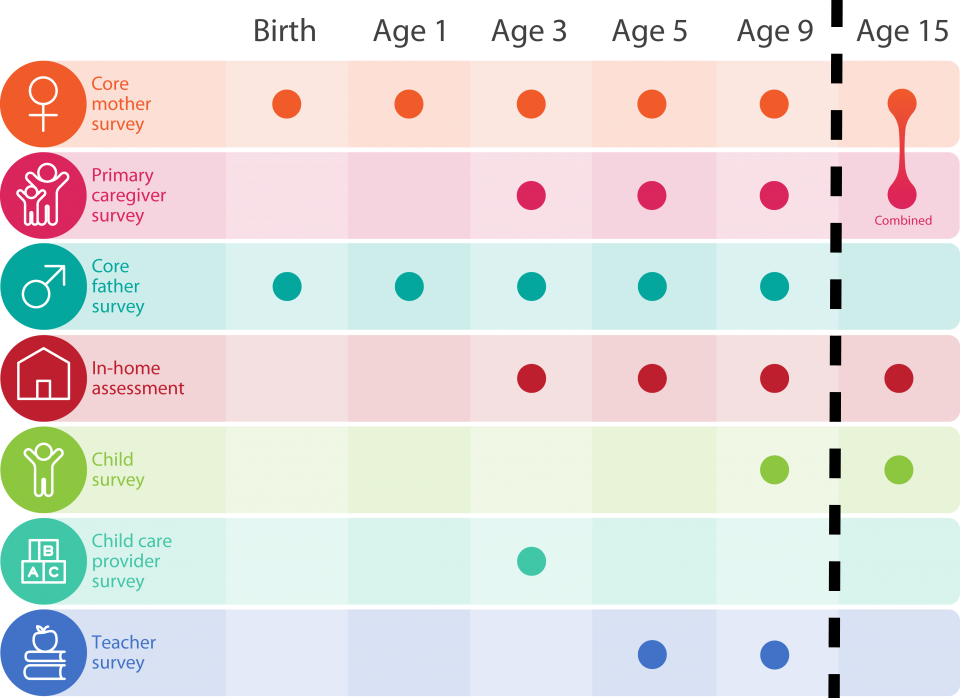
\includegraphics[width=\textwidth]{figures/ff_design_public2}
\end{center}

\end{frame}
%%%%%%%%%%%%%%%%%%%%%%%%%
\begin{frame}

\begin{center}
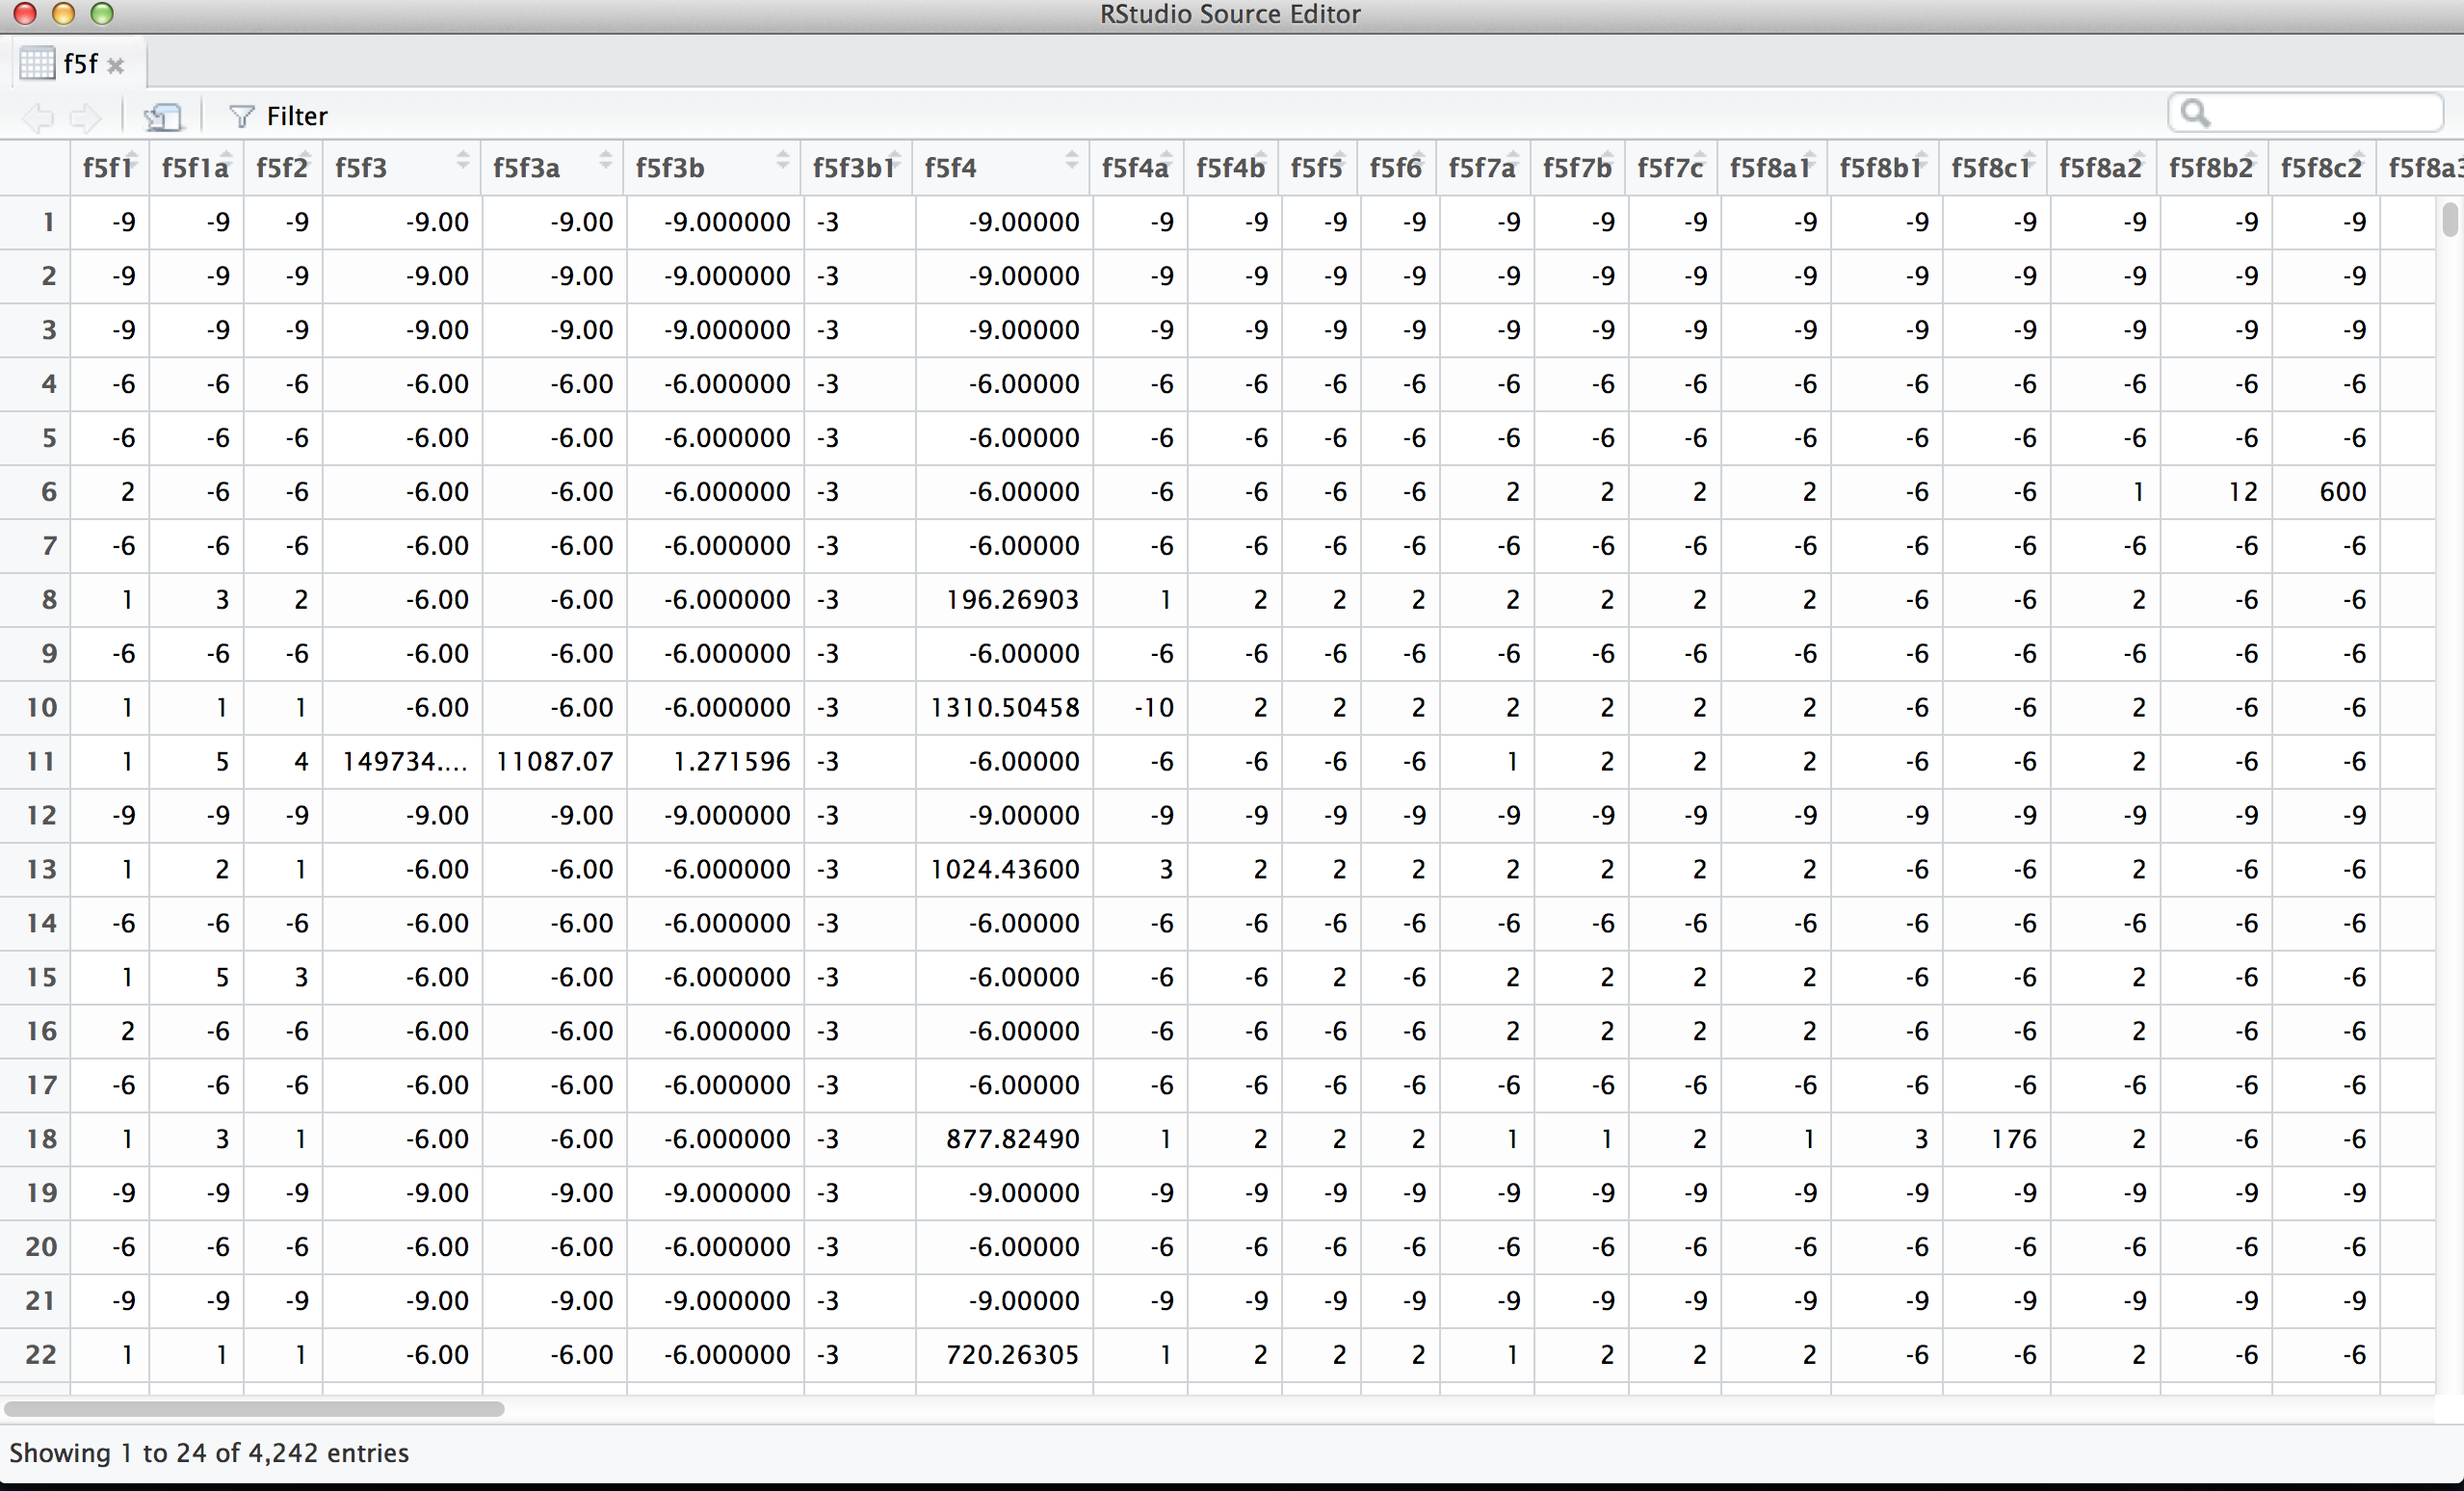
\includegraphics[width=\textwidth]{figures/ffc_rawdata_f5f}
\end{center}

\end{frame}
%%%%%%%%%%%%%%%%%%%%%%%%%
\begin{frame}

\begin{center}
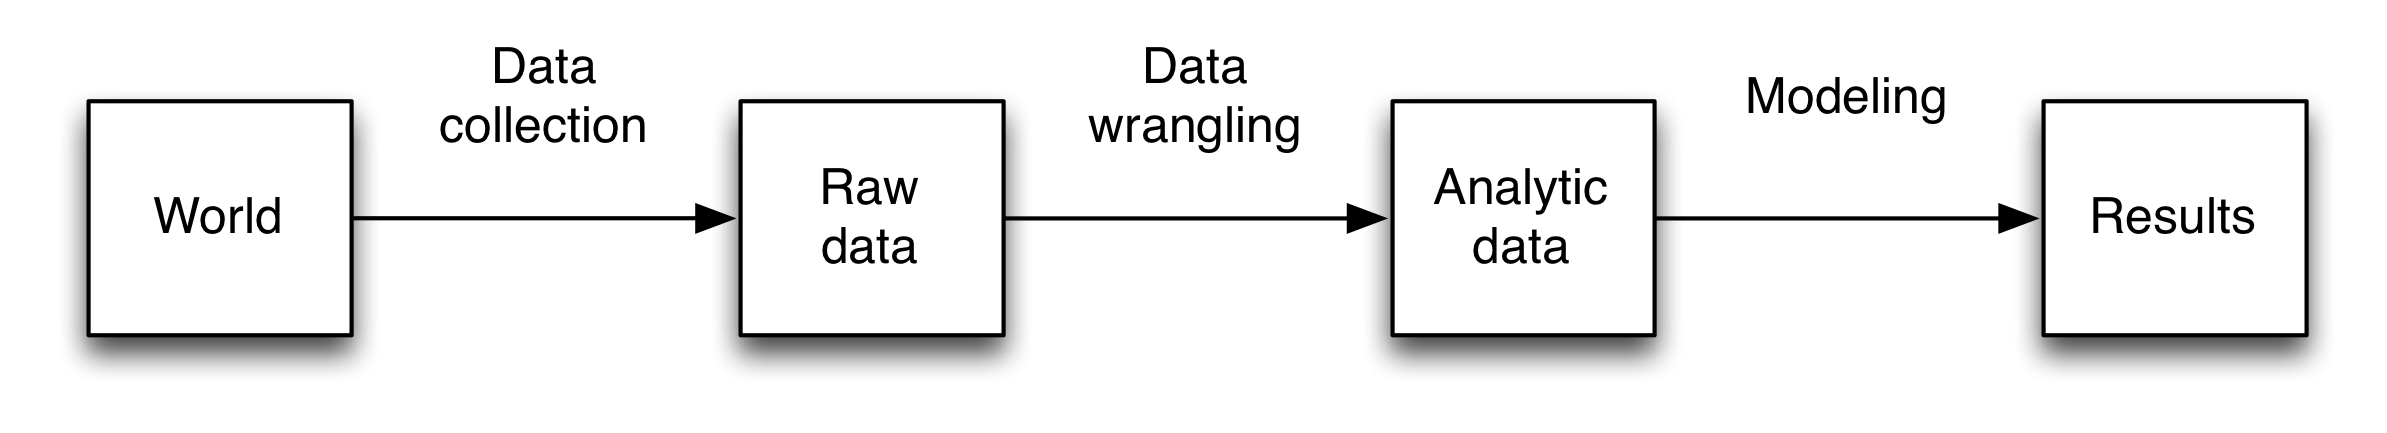
\includegraphics[width=\textwidth]{figures/scientific_pipeline}
\end{center}

\end{frame}
%%%%%%%%%%%%%%%%%%%%%%%%%
\begin{frame}

How do I know what these variables are? 

\begin{center}
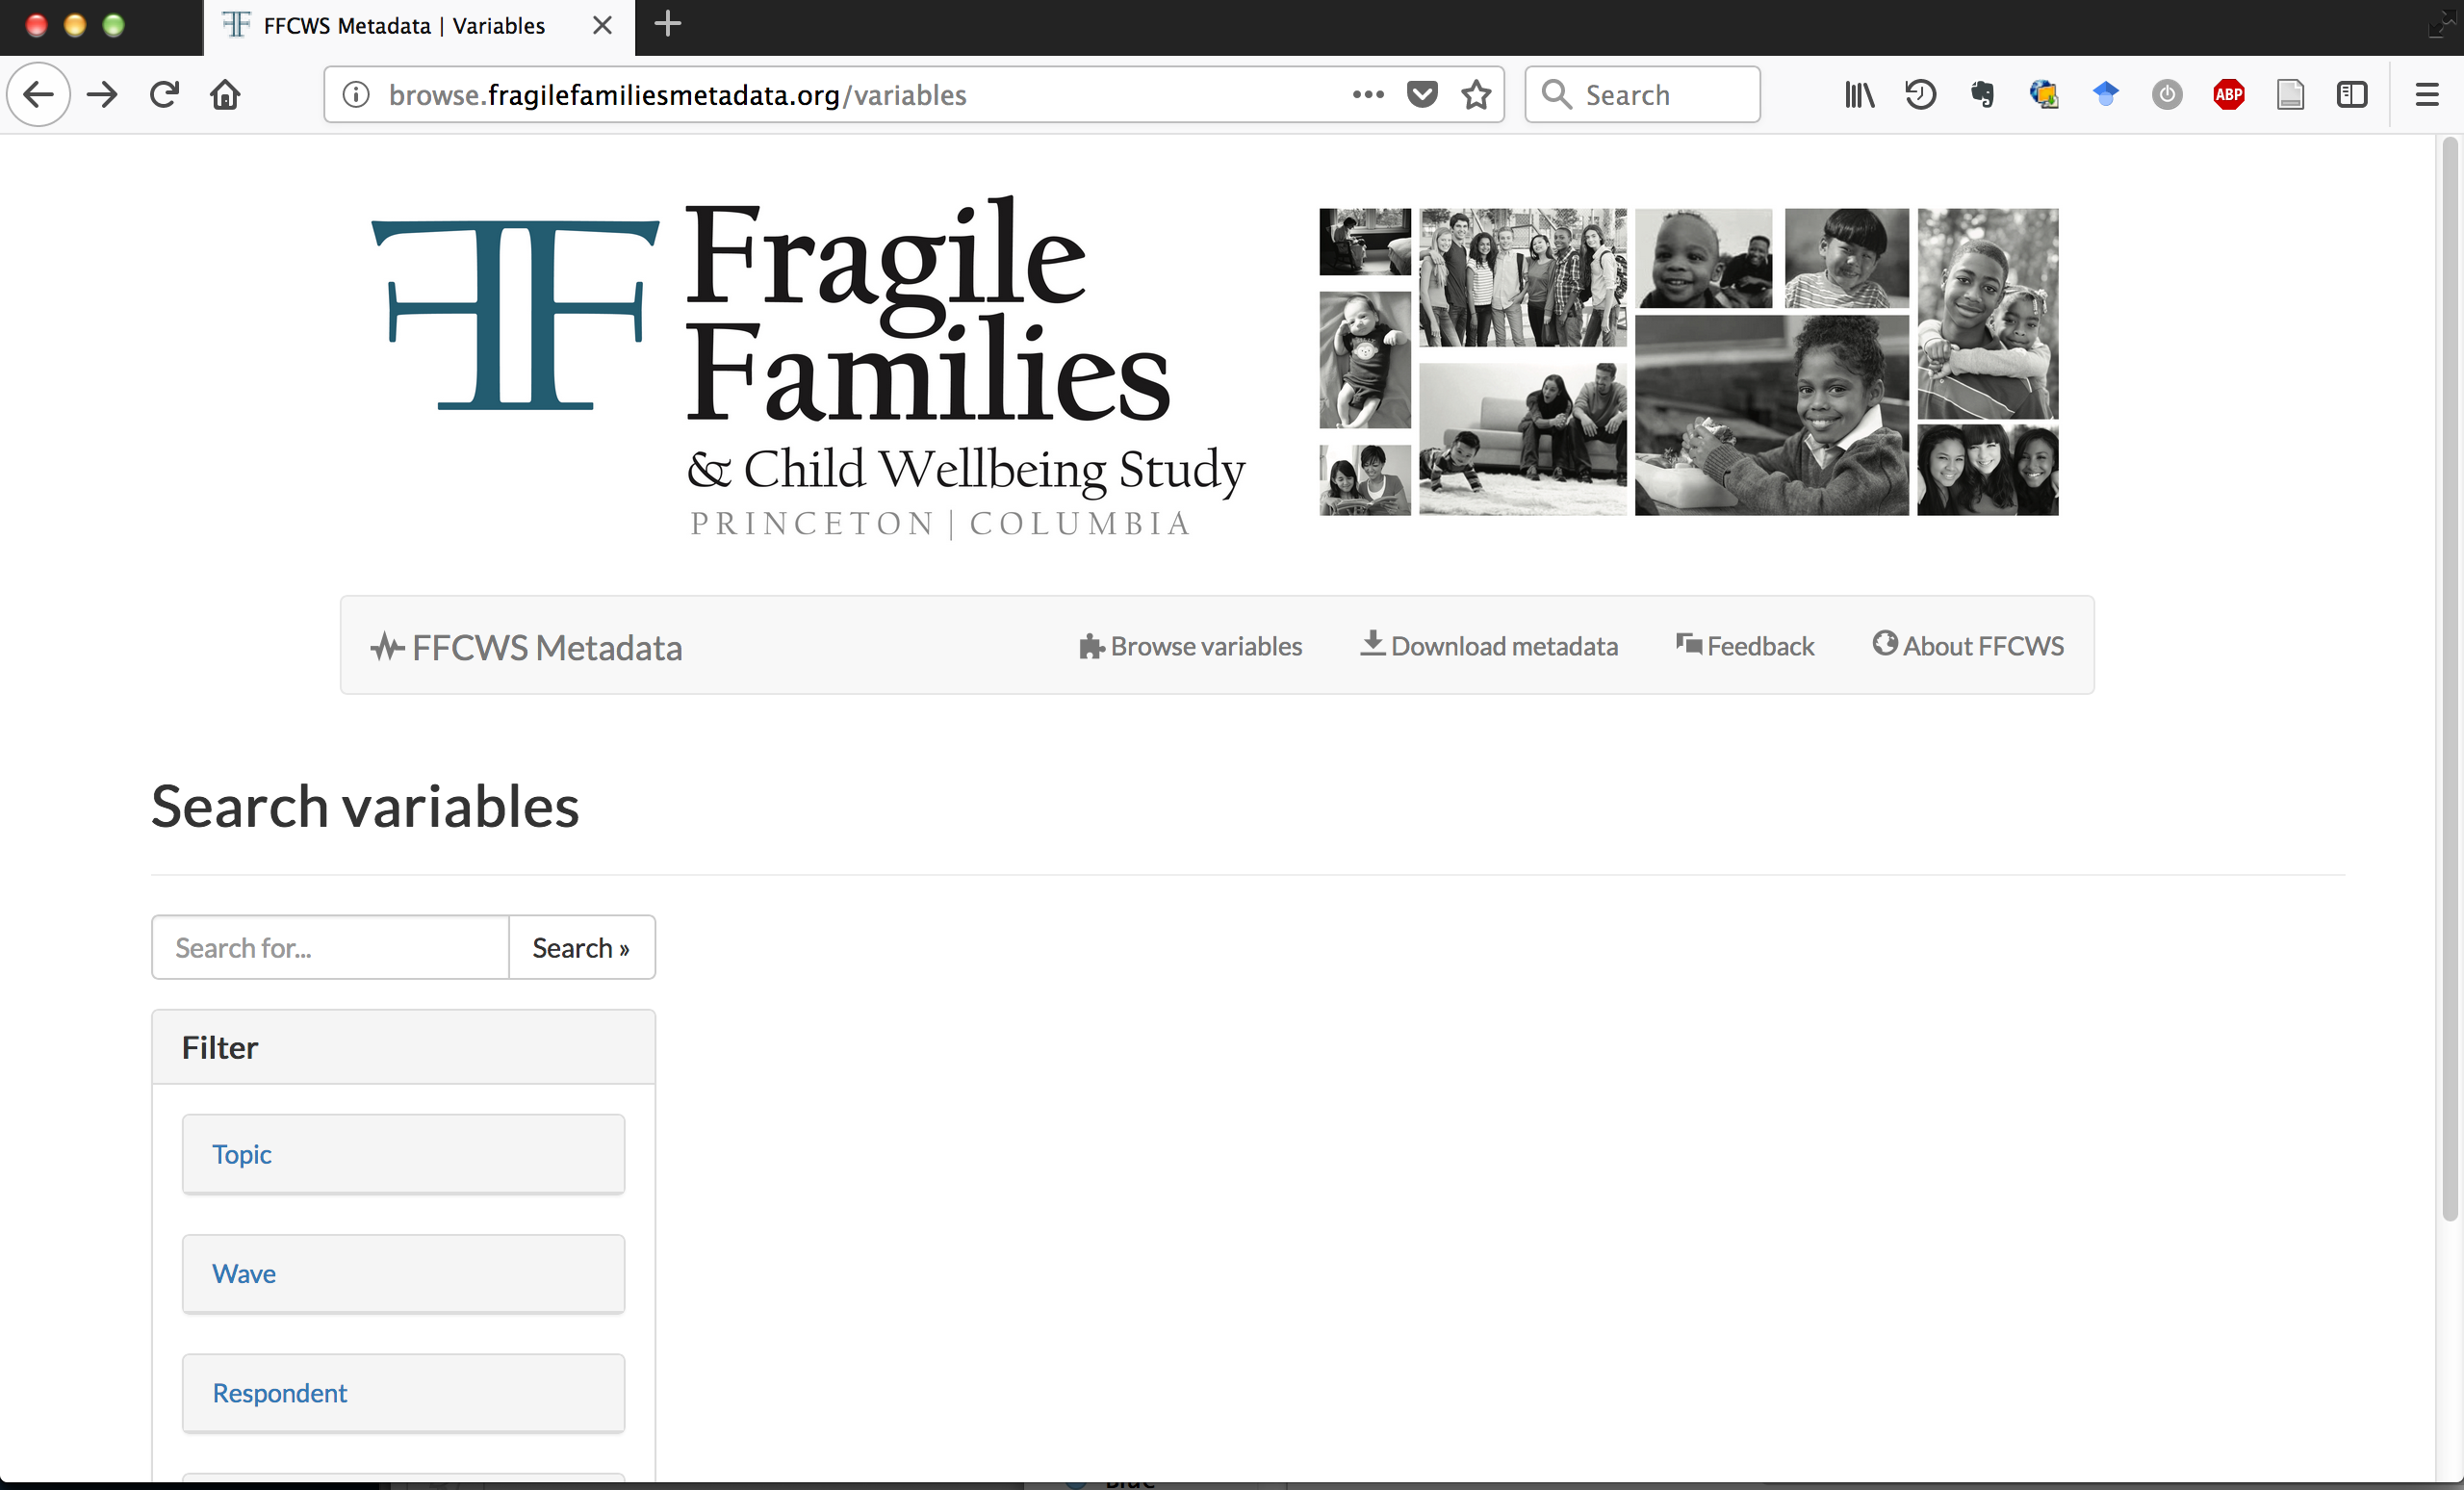
\includegraphics[width=\textwidth]{figures/ff_metadata_browser}
\end{center}

\vfill

\url{http://metadata.fragilefamilies.princeton.edu/variables}

\end{frame}
%%%%%%%%%%%%%%%%%%%%%%%%%%%
\begin{frame}

Introducing \texttt{cm1relf}\\

\url{http://metadata.fragilefamilies.princeton.edu/variables/cm1relf}

\end{frame}
%%%%%%%%%%%%%%%%%%%%%%%%%%%
\begin{frame}

You can filter variables by:
\begin{itemize}
\item Topic
\item Wave
\item Respondent
\item Variable Type (e.g., continuous, ordered categorical, unordered categorical, etc).
\end{itemize}

\end{frame}	
%%%%%%%%%%%%%%%%%%%%%%%%%%%
\begin{frame}

Why \texttt{cm1relf}? \pause

\begin{center}
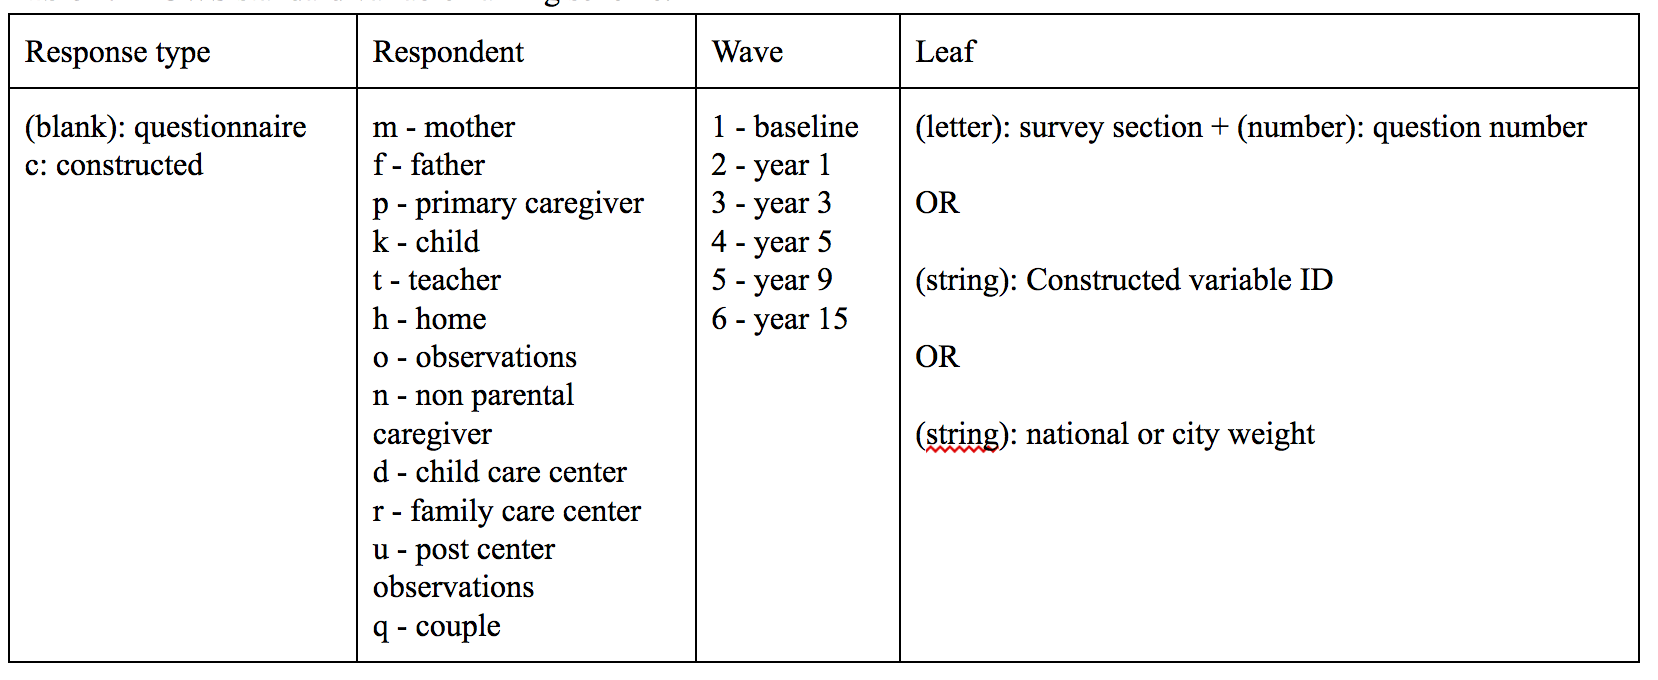
\includegraphics[width=\textwidth]{figures/ff_variablename_standards}
\end{center}

\end{frame}
%%%%%%%%%%%%%%%%%%%%%%%%%%
\begin{frame}

Want direct access to the metadata?  \pause No problem

\begin{itemize}
\item API: \url{api.metadata.fragilefamilies.princeton.edu}
\item Python package: \url{github.com/fragilefamilieschallenge/ffmetadata-py}
\item R package: \url{github.com/fragilefamilieschallenge/ffmetadata}
\item Raw metadata: \url{api.fragilefamiliesmetadata.org/get_metadata}
\end{itemize}

\end{frame}
%%%%%%%%%%%%%%%%%%%%%%%%%%%
\begin{frame}

\centering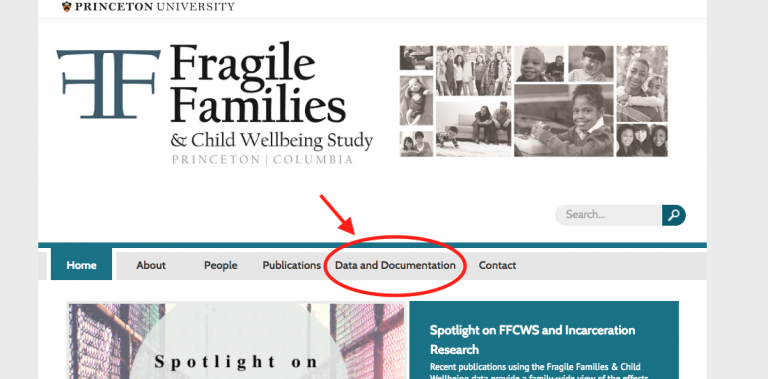
\includegraphics[width = .8\textwidth]{figures/Doc1}

\end{frame}
%%%%%%%%%%%%%%%%%%%%%%%%%%%
\begin{frame}

\centering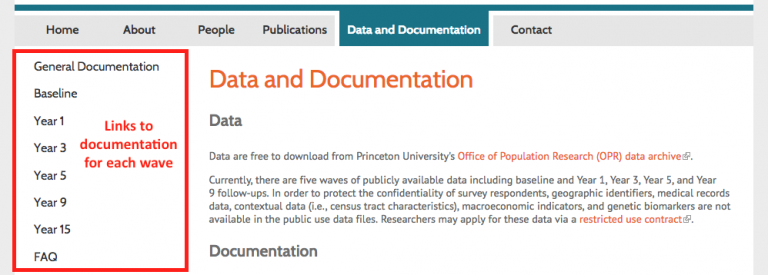
\includegraphics[width = .8\textwidth]{figures/Doc2}

\end{frame}
%%%%%%%%%%%%%%%%%%%%%%%%%%%
\begin{frame}

\centering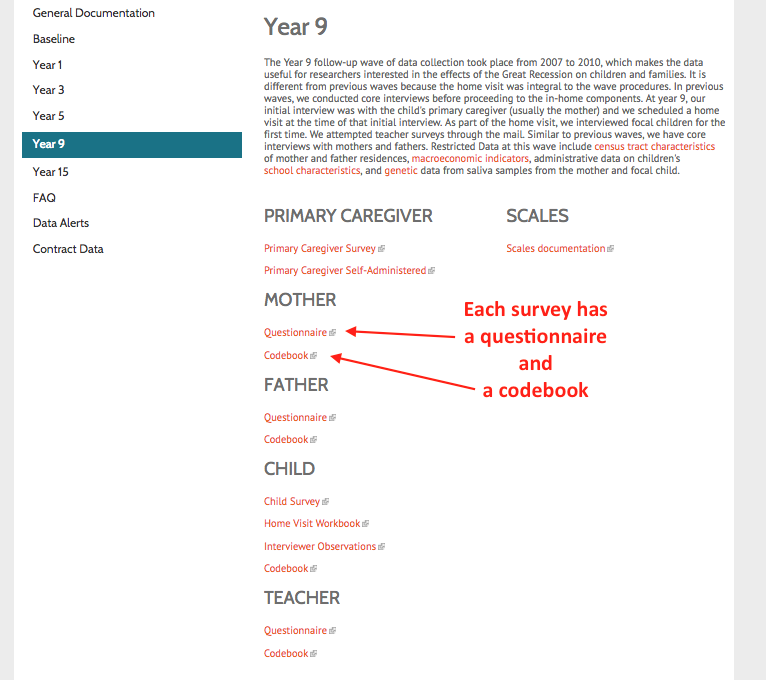
\includegraphics[width = .8\textwidth]{figures/Doc3}

\end{frame}
%%%%%%%%%%%%%%%%%%%%%%%%%%%
\begin{frame}

Questionnaire:\\
\centering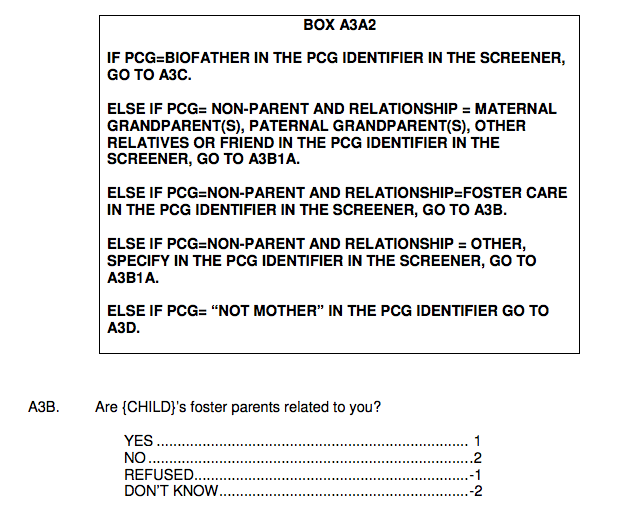
\includegraphics[width = .8\textwidth]{figures/Doc4}

\end{frame}
%%%%%%%%%%%%%%%%%%%%%%%%%%%
\begin{comment}
\begin{frame}

In the corresponding codebook, we see the count of respondents who gave each answer:
\vskip .3cm
\begin{center}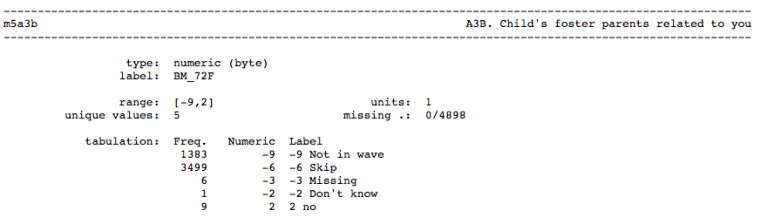
\includegraphics[width = .8\textwidth]{figures/Doc5}\end{center}
\vskip .3cm \pause
Things to note here:
\vskip .3cm \pause
\begin{itemize}
\item The question referred to in the questionnaire as A3B is called m5a3b in the codebook. \pause
\item There are missing codes.
\end{itemize}

\end{frame}
\end{comment}
%%%%%%%%%%%%%%%%%%%%%%%%%%%
\begin{frame}

\begin{center}
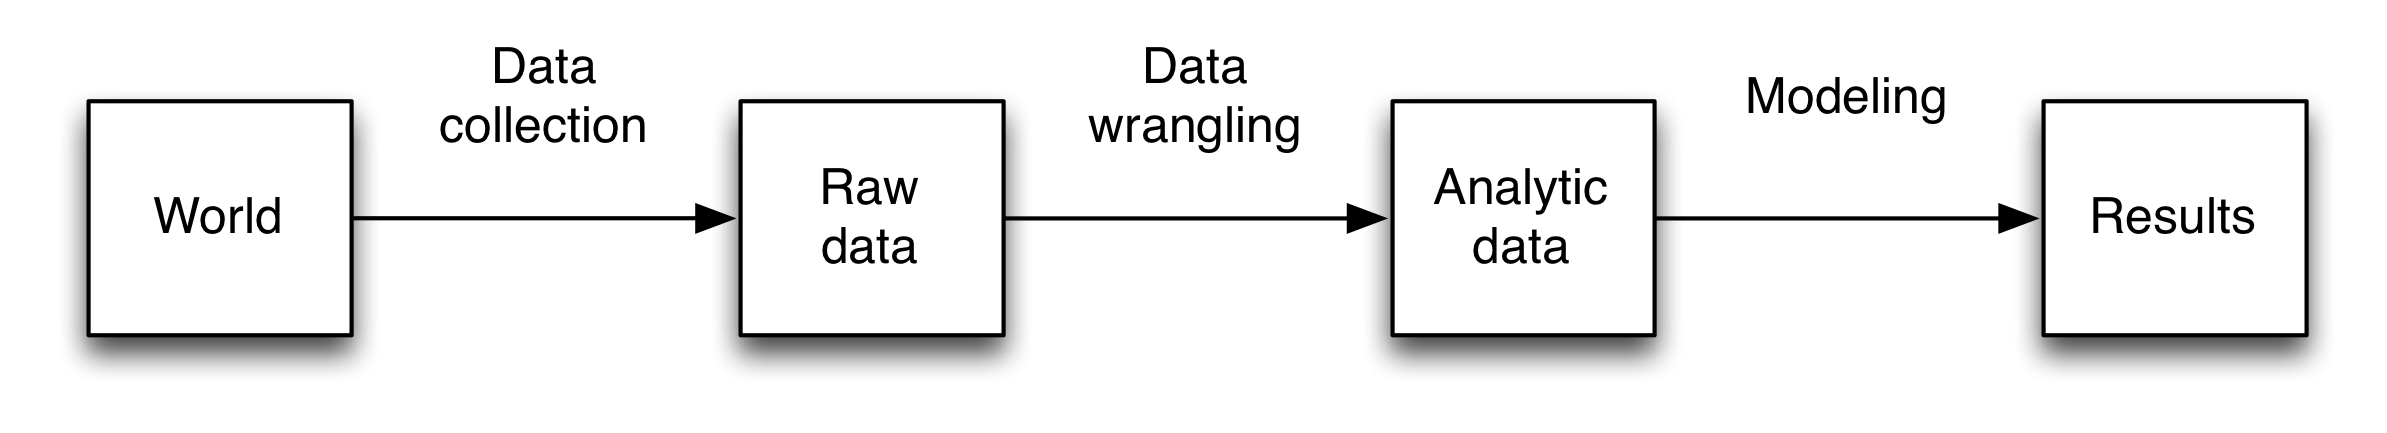
\includegraphics[width=\textwidth]{figures/scientific_pipeline}
\end{center}

\end{frame}
%%%%%%%%%%%%%%%%%%%%%%%%%
\begin{frame}
\frametitle{Building a submission}

Submissions include:
\begin{enumerate}
\item Predictions
\item Code
\item Narrative explanation
\end{enumerate}

\vfill
Submission preparation instructions: \textcolor{blue}{\href{http://www.fragilefamilieschallenge.org/upload-your-contribution/}{www.fragilefamilieschallenge.org/upload-your-contribution/}}

\end{frame}
%%%%%%%%%%%%%%%%%%%%%%%%%%%
\begin{frame}{Get on the leaderboard}

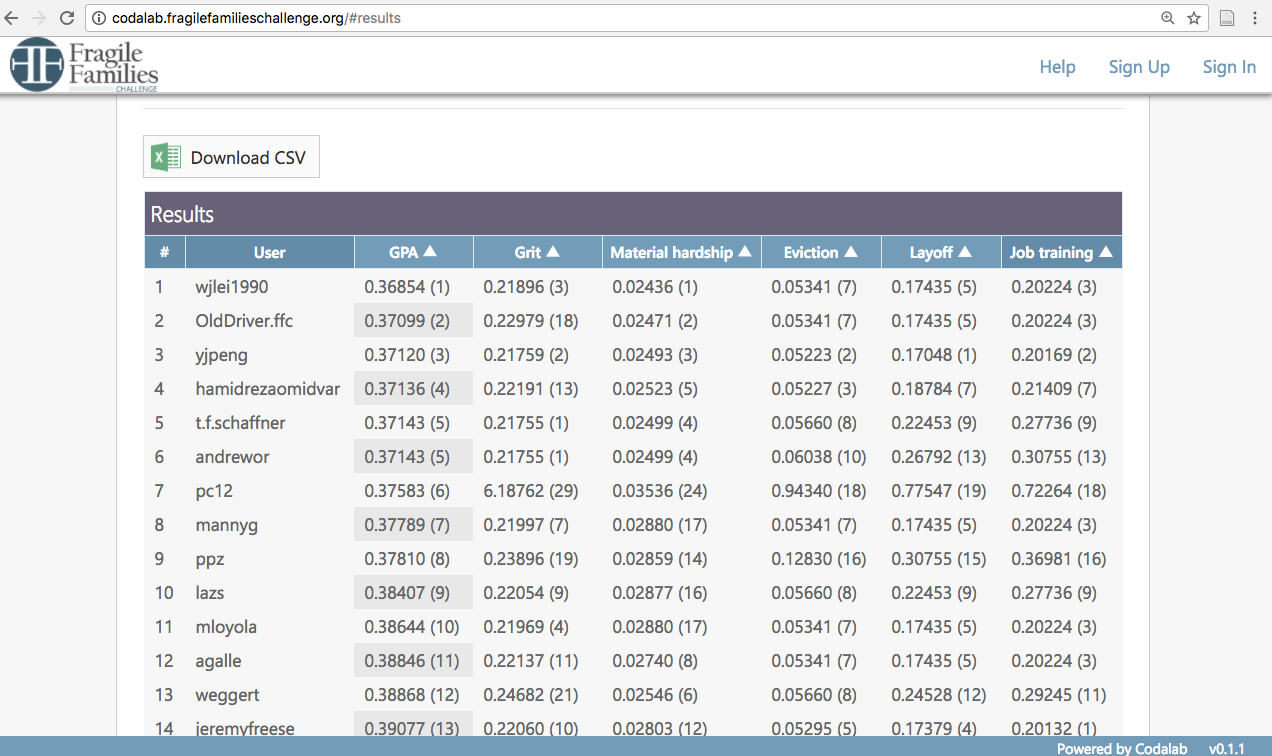
\includegraphics[width = \textwidth]{figures/leaderboard}

\end{frame}
%%%%%%%%%%%%%%%%%%%%%%%%%%%
\begin{frame}

\begin{center}
\LARGE{Advice}
\end{center}

\end{frame}
%%%%%%%%%%%%%%%%%%%%%%%%%%%
\begin{frame}

Most good approaches will likely involve \pause
\begin{itemize}
\item careful data preparation
\pause
\item flexible models that avoid overfitting
\end{itemize}

\end{frame}
%%%%%%%%%%%%%%%%%%%%%%%%%%%
\begin{frame}{Common missing codes\footnote{For more complete list and explanation, see \url{http://www.fragilefamilieschallenge.org/missing-data/}\vskip .2cm}}

Not all missing data is the same
\begin{small}
\begin{itemize}
\item -9 Not in wave - Did not participate in survey/data collection component
\item -6 Valid skip - Intentionally not asked question; question does not apply to respondent or response known based on prior information.
\item -2 Don't know - Respondent asked question; responded ``Don't Know''.
\item -1 Refuse - Respondent asked question; refused to answer question
\item NA also used occasionally
\end{itemize}
\end{small}

\end{frame}
%%%%%%%%%%%%%%%%%%%%%%%%%%%
\begin{frame}

How can you optimally combine human and machine effort? \\ \pause
\begin{itemize}
\item automatic feature selection
\item human-assisted automatic feature selection 
\item computer-assisted human feature selection
\item some other hybrid
\end{itemize}

\end{frame}
%%%%%%%%%%%%%%%%%%%%%%%%%%%
\begin{frame}

Fragile Families Challenge:
\begin{enumerate}
\item common task method
\pause
\item use submissions to do cool stuff
\end{enumerate}

\end{frame}
%%%%%%%%%%%%%%%%%%%%%%%%%%%
\begin{frame}

\begin{center}
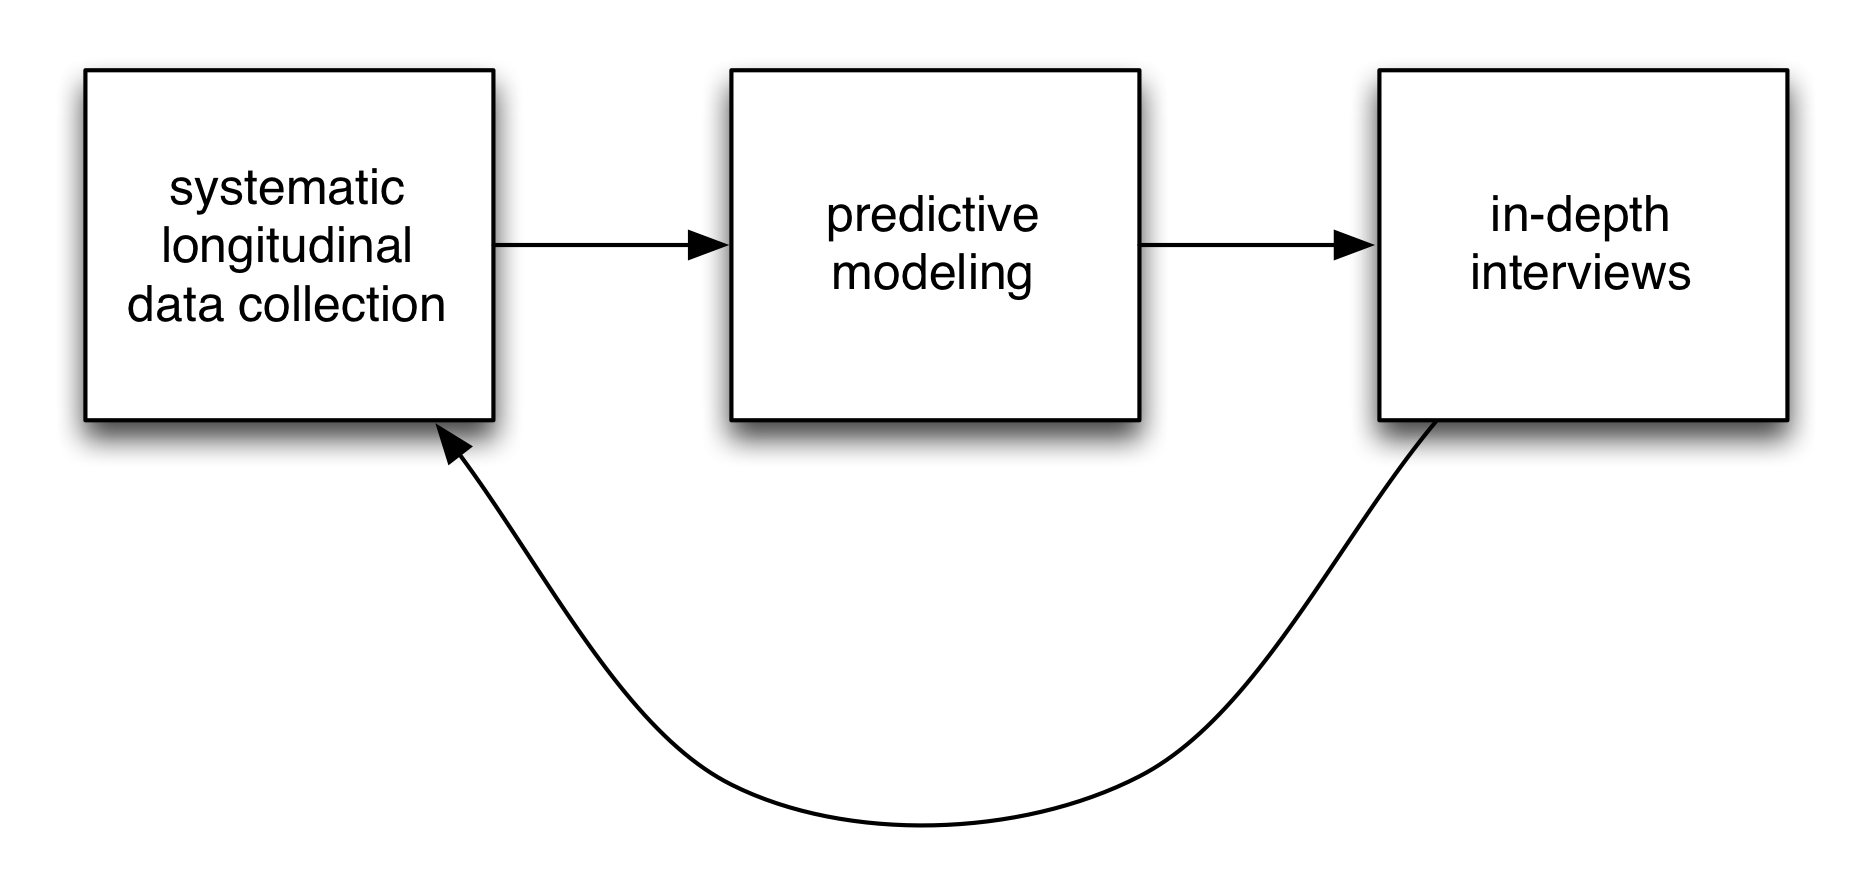
\includegraphics[width=\textwidth]{figures/kaizen_cycle}
\end{center}

\end{frame}
%%%%%%%%%%%%%%%%%%%%%%%%%%%
\begin{frame}

Next steps:
\begin{itemize}
\item One big paper with hundreds of authors \pause
\item Special issue of \textit{Socius} \pause
\item Our papers: \pause
\begin{itemize}
\item ``Privacy, ethics, and high-dimensional social science data: A case study of the Fragile Families Challenge'' \pause
\item ``Making the analysis of complex survey data more efficient, reliable, and enjoyable: A case study from the Fragile Families Challenge'' \pause
\item ``Computational reproducibility and the Fragile Families Challenge: Empirical results, lessons learned, and suggestions for the future'' \pause
\end{itemize}
\item We are currently conducting in-depth interviews in three cities
\end{itemize}

\end{frame}
%%%%%%%%%%%%%%%%%%%%%%%%%%%%%%%%%%%%%%%%%%%%%%%%%%%%%%%%
\begin{frame}

\begin{center}
\LARGE Questions
\end{center}

\end{frame}
%%%%%%%%%%%%%%%%%%%%%%%%%%%%%%%%%%%%%%%%%%%%%%%%%%%%%%%%





\end{document}